\documentclass[twoside]{article}
\usepackage[accepted]{aistats2e}

\usepackage[numbers]{natbib}

\usepackage{color}
\usepackage{latexsym}
\usepackage{amsmath,amssymb,amsthm,amsfonts}
\usepackage{algorithm,algorithmic}
\usepackage{graphicx,subfigure}

%\usepackage[accepted]{aistats2e}

% If your paper is accepted, change the options for the package
% aistats2e as follows:
%
%\usepackage[accepted]{aistats2e}
%
% This option will print headings for the title of your paper and
% headings for the authors names, plus a copyright note at the end of
% the first column of the first page.


\begin{document}

% If your paper is accepted and the title of your paper is very long,
% the style will print as headings an error message. Use the following
% command to supply a shorter title of your paper so that it can be
% used as headings.
%
%\runningtitle{I use this title instead because the last one was very long}

% If your paper is accepted and the number of authors is large, the
% style will print as headings an error message. Use the following
% command to supply a shorter version of the authors names so that
% they can be used as headings (for example, use only the surnames)
%
%\runningauthor{Surname 1, Surname 2, Surname 3, ...., Surname n}

\twocolumn[

\aistatstitle{On Learning Discrete Graphical Models using Group-Sparse Regularization}

\aistatsauthor{Ali Jalali \And Pradeep Ravikumar \And Vishvas Vasuki \And Sujay Sanghavi}

\aistatsaddress{ECE, UT Austin \\ \texttt{alij@mail.utexas.edu} \And CS, UT Austin\\ \texttt{pradeepr@cs.utexas.edu} \And CS, UT Austin\\ \texttt{vvasuki@cs.utexas.edu} \And ECE, UT Austin\\\texttt{sanghavi@mail.utexas.edu}}]


\bibliographystyle{plainnat}

%%%%% MACROS %%%%%


\newtheorem{lemma}{Lemma}
\newtheorem{definition}{Definition}
\newtheorem{proposition}{Proposition}
\newtheorem{theorem}{Theorem}

\newenvironment{carlist}
{\begin{list}{$\bullet$}
{\setlength{\topsep}{0in} \setlength{\partopsep}{0in}
 \setlength{\parsep}{0in} \setlength{\itemsep}{\parskip}
 \setlength{\leftmargin}{0.07in} \setlength{\rightmargin}{0.08in}
 \setlength{\listparindent}{0in} \setlength{\labelwidth}{0.08in}
 \setlength{\labelsep}{0.1in} \setlength{\itemindent}{0in}}}
{\end{list}}

\newcommand\inner[1]{\left\langle #1 \right\rangle}
\newcommand\myparagraph[1]{\noindent {\it #1.}}
%\newcommand{\myparagraph}[1]{\noindent \paragraph{#1}}
\newcommand{\comment}[1]{}
\newcommand{\tr}[2]{\left<#1,#2\right>}
\newcommand{\matnorm}[2]{|\!|\!|#1|\!|\!|_{#2}}
\newcommand{\norm}[2]{\left\|#1\right\|_{#2}}
\newcommand{\flaten}[1]{\mathbf{v}\left(#1\right)}

\def\Data{\mathcal{D}}
\def\M{\mathcal{M}}
\def\N{\mathcal{N}}
\def\A{\mathcal{A}}
\def\X{\mathcal{X}}
\def\I{\mathcal{I}}
\def\J{\mathcal{J}}
\def\real{\mathbb{R}}
\def\reals{\mathbb{R}}
\def\pdim{p}
\def\mdim{m}
\def\kdim{k}
\def\numobs{n}
\def\Data{D}
\def\regpar{\lambda}
\def\vertex{V}
\def\edge{E}
\def\statenum{m}
\def\svert{\ensuremath{r}}
\def\defn{:=}
\def\fisher{Q}
\def\support{S}
\def\dual{Z}
\def\graph{G}
\def\degmax{d}
\def\order{\mathcal{O}}
\def\mprob{\mathbb{P}}
\def\defn{:=}
\def\maxcliquesize{c}

\begin{abstract}
Social network analysis has attracted increasing attention in recent years. In many social networks, besides friendship links amongst users, the phenomenon of users associating themselves with groups or communities is common. Thus, two networks exist simultaneously: the friendship network among users, and the affiliation network between users and groups. In this paper, we tackle the affiliation recommendation problem, where the task is to predict or suggest new affiliations between users and communities, given the current state of the friendship and affiliation networks. More generally, affiliations need not be community affiliations - they can be a user's taste, so affiliation recommendation algorithms have applications beyond community recommendation. In this paper, we show that information from the friendship network can indeed be fruitfully exploited in making affiliation recommendations. Using a simple way of combining these networks, we suggest two models of user-community affinity for the purpose of making affiliation recommendations: one based on graph proximity, and another using latent factors to model users and communities. We explore the two classes of affiliation recommendation algorithms suggested by these models. We evaluate these algorithms on two real world networks - Orkut and Youtube. In doing so, we motivate and propose a way of evaluating recommenders, by measuring how good the top 50 recommendations are for the average user, and demonstrate the importance of choosing the right evaluation strategy. The algorithms suggested by the graph proximity model turn out to be the most effective and efficient. This use of link prediction techniques for the purpose of affiliation recommendation is, to our knowledge, novel.

\end{abstract}

\section{Introduction}

\myparagraph{Markov Random Fields and Structure Learning} Undirected graphical models, also known as Markov random fields, are used in a variety of domains, including statistical
physics~\citep{Ising25}, natural language processing~\citep{Manning:99}, image analysis~\citep{Woods78,Hassner80,Cross83}, and spatial
statistics~\citep{Ripley81}, among others. A Markov random field (MRF) over a $\pdim$-dimensional discrete random vector $X = (X_1, X_2,\ldots,X_p)$ is specified by an undirected graph $\graph = (\vertex, \edge)$, with vertex set $\vertex = \{1, 2, \ldots, \pdim \}$ -- one for each variable -- and edge set $\edge \subset \vertex \times \vertex$.  The structure of this graph encodes certain conditional independence assumptions among subsets of the variables. In this paper, we consider the task of structure learning, i.e.  estimating the underlying graph structure associated with a general discrete Markov random field from $\numobs$ independent and identically distributed samples $\{ x^{(1)}, x^{(2)}, \ldots, x^{(\numobs)} \}$.

\myparagraph{High-dimensional setting and Group sparsity} We are interested in structure learning in the setting where the dimensionality $p$ of the data is larger than the number of samples $n$. While classical procedures typically break down under such high-dimensional scaling, an active line of recent research has shown it is still possible to obtain practical consistent procedures by leveraging low-dimensional structure. The most popular example is that of leveraging sparsity using $\ell_1$-regularization (e.g.,~\cite{CandesTao06,Donoho:Elad:03,Meinshausen:06,ng:04,Tropp:06,Wainwright06_new,ZhaoYu06}). For MRF structure learning, such $\ell_1$-regularization has been successfully used for Gaussian \cite{Meinshausen:06} and discrete binary pairwise (i.e. Ising) models \citep{RWLIsing,LeeKoller07}. In these instances, there is effectively only one parameter per edge, so that a sparse graph corresponds to a sparse set of parameters. In this paper, we are interested in more general discrete graphical models -- where each variable can take $m$ possible values, and factors can be of order higher than two. We now have multiple parameters per edge, and thus the relevant low-dimensional structure is that of {\em group sparsity}: all parameters of an edge form a group, and a sparse graph now corresponds to certain \emph{groups of parameters} being non-zero. The counterpart of $\ell_1$ regularization for such group-sparse structure is $\ell_1/\ell_q$ regularization for $q > 1$, where we collate the $\ell_q$ norms of the groups, and compute their overall $\ell_1$ norm. Recent work on group and block-sparse linear regression \citep{TurlachVW, ZH08,NWJoint,Lounici09,Obozinski10,RLLWSPAM,BachMKL} show that under such group-sparse settings, group-sparse regularization outperforms the use of $\ell_1$ penalization.

\myparagraph{Our Results: Pairwise $m$-ary models} In this paper, we provide a quantitative consistency analysis of group-sparse regularized structure recovery for general discrete graphical models. We first consider the case of pairwise but otherwise $m$-ary discrete graphical models, and analyze a group-sparse variant of the procedures in ~\citep{RWLIsing,Meinshausen:06}: for each vertex $\svert \in V$, we estimate its neighborhood set using $\ell_1/\ell_2$-regularized maximum conditional likelihood. This reduces to multi-class logistic regression, for which we characterize the number of samples needed for \emph{sparsistency} $i.e.$ consistent recovery of the group-support-set with high probability. This analysis extends recent high-dimensional analyses for linear models to logistic models, and is of independent interest even outside the context of graphical models. We then combine the neighborhood sets across vertices to form the graph estimate. There has been a strong line of work on developing fast algorithms to solve these sparse multiclass logistic regression programs including ~\citet{MGB08,KCFH05}. Indeed, \citep{Dahinden07,Dahinden10} show good empirical performance using such $\ell_1/\ell_q$ regularization even with the joint likelihood over all variables.

\myparagraph{Our Results: General $m$-ary models} One (natural, but expensive)  extension to graphical models with higher-order factors is to again use group-sparse regularization but with higher order factors as groups. However, this leads to prohibitive computational complexity -- e.g. there are $\order(\pdim^{c})$ possible factors of order $c$. Indeed, in their empirical study of such regularizations, \citet{Dahinden07,Dahinden10} could scale up to small graph sizes, even while using some intelligent heuristics. This motivates our second main result. Suppose we solve the pairwise graphical model estimation problem, even when the true model has higher order factors. What is the relationship of this estimate with the true underlying graph? We investigate this for {\em hierarchical} graphical models where the absence of any lower-order factor also implies the absence of factors over supersets of the lower-order factor variables. Higher-order factors could, in principle, cause our pairwise estimator to include spurious edges. Surprisingly, we obtain the result that under slightly more stringent assumptions on the scaling of the sample size (dependent on the size of the higher-order factors) the pairwise estimator excludes the irrelevant edges, and includes all ``dominant'' pairwise edges whose parameters are larger than a certain threshold that depends on the size of the parameters values of higher-order factors. As a consequence, if all pairwise effects are dominant enough, we recover the graph exactly even while using a simple pairwise estimator. But even otherwise, the guaranteed false edge exclusion could be used for further greedy procedures, though we defer further discussion in the sequel.

\myparagraph{Existing approaches} Methods for estimating such graph structure include those based on constraint and hypothesis testing~\citep{spirtes:00}, and those that estimate restricted classes of graph structures such as trees~\citep{chowliu:68}, polytrees~\cite{dasgupta:99}, and hypertrees~\citep{srebro:03}. Another class of approaches estimate the local neighborhood of each node via exhaustive search for the special case of bounded degree graphs. Abbeel et al.\cite{AbbKolNg06} propose a method for learning factor graphs based on local conditional entropies and thresholding, but the computational complexity grows at least as quickly as $\order(\pdim^{\degmax+1})$, where $\degmax$ is the maximum neighborhood size in the graphical model. Bresler et al.~\cite{Bresler08} describe a related local search-based method, and prove under relatively mild assumptions that it can recover the graph structure with $\Theta(\log \pdim)$ samples. However, in the absence of additional restrictions, the computational complexity of the method is $\order(\pdim^{\degmax+1})$. Csisz\'{a}r and Talata~\cite{Csiszar:06} show consistency of a method that uses pseudo-likelihood and a modification of the BIC criterion, but this also involves a prohibitively expensive search.

% \myparagraph{Existing approaches} Methods for estimating such graph structure include those based on constraint and hypothesis testing~\citep{spirtes:00}: these estimate conditional
% independencies from the data, and then determine a graph that most closely represents those independencies. Another class of score-based approaches 
% search through a set of candidate graph structures, but unfortunately these are typically NP-hard~\cite{chickering:95}. Indeed, for general undirected graphical models with discrete random variables, calculation of the partition function or cumulant function associated with the Markov random field function is computationally intractable~\cite{Welsh93}. This motivated 
% estimating restricted classes of graph structures such as trees~\citep{chowliu:68}, polytrees~\cite{dasgupta:99}, and hypertrees~\citep{srebro:03}. 
% Another class of approaches is based on estimating the local neighborhood of each node via exhaustive search for the special case of bounded degree graphs. Abbeel et al.\cite{AbbKolNg06} 
% propose a method for learning factor graphs based on local conditional entropies and thresholding, and analyze its behavior in terms of Kullback-Leibler divergence between the fitted and true models. 
% They obtain a sample complexity that grows logarithmically in the number of vertices $\pdim$, but the computational complexity grows at least as quickly as $\order(\pdim^{\degmax+1})$, where $\degmax$ is the maximum neighborhood size in the graphical model. This order of complexity arises from the fact that for each node, there are $\binom{\pdim}{\degmax} = \order(\pdim^\degmax)$
% possible neighborhoods of size $\degmax$ for a graph with $\pdim$ vertices. Bresler et al.~\cite{Bresler08} describe a related simple search-based method, and prove under relatively mild assumptions that it can recover the graph structure with $\Theta(\log \pdim)$ samples. However, in the absence of additional restrictions, the computational complexity of the method is $\order(\pdim^{\degmax+1})$. Csisz\'{a}r and Talata~\cite{Csiszar:06} show consistency of a method that uses pseudo-likelihood and a modification of the BIC criterion, but this also involves a prohibitively expensive search. 

%\citet{BachHMKL08} propose and analyze a greedy active-set algorithm for solving group-sparse regularized estimators, for the case where the features (sufficient statistics of the graphical model in our case) are drawn from a RKHS corresponding to an amenable hierarchical set of kernels.

%% Shrug off structured group-sparse variants
%It also remains to investigate the consequences and extensions of our analysis on structured variants of group-sparse regularizations such as the hierarchical Composite Absolute Penalties (CAP) family~\citep{ZRYCAP}, structured sparsity~\citep{HZM09} and hierarchical multiple kernel learning~\citep{BachHMKL08}.


\def\CliqueSet{\mathcal{C}}
\def\clique{C}

\section{Problem Setup and Notation}

\myparagraph{MRFs and their Parameterization} We consider the task of estimating the graph structure associated with a general discrete Markov random field. Let $X = (X_1,\hdots,X_p)$ be a random vector, each variable $X_i$ taking values in a discrete set $\mathcal{X}= \{1,2, \ldots, \statenum\}$ of cardinality $m$. Let $G = (V,E)$ denote a graph with $p$ nodes,  corresponding to the $p$ variables $\{X_1,\hdots,X_p\}$. Let $\CliqueSet$ be a set of cliques (fully-connected subgraphs) of the graph $G$, and let $\{ \phi_{\clique} : \mathcal{X}^{|\clique|} \mapsto \real, \; \clique \in \CliqueSet \}$ be a set of ``clique potential'' functions. With this notation, the distribution of $X$ takes the form
\begin{eqnarray}
\label{EqnGenMRFPot}
\mprob(x) & \propto & \exp \left \{\sum_{\clique \in \CliqueSet} \phi_\clique(x_\clique) \right \}.
\end{eqnarray}
\noindent Since $\mathcal{X}$ is discrete, each potential function $\phi_{\clique}$
can be parameterized as linear combinations of $\{0,1\}$-valued indicator functions -- one for each configuration of $x_\clique$.  
For each $s \in \vertex$ and $j \in \{1, \ldots, \statenum-1\}$, we can define node-wise indicators, 
\begin{eqnarray*}
\I[x_{s} = j] & = & \begin{cases} 1 & \mbox{if $x_s =j$} \\ 
											0 & \mbox{otherwise.}
                    \end{cases}
\end{eqnarray*}
Note that we omit an indicator for $x_s = \statenum$ from the list, since
it is redundant given the indicators for $j = 1, \ldots, \statenum-1$.
In a similar fashion, we can define the $|\clique|$-way clique-wise indicator functions 
$\I[x_\clique = v]$, for $v \in \{1,2,\ldots, \statenum - 1\}^{|\clique|}$.

\noindent With this notation, any set of potential functions can then be written as
\begin{eqnarray*}
\phi_{\clique}(x_\clique) & = & \sum_{v \in \{1, \ldots, \statenum-1 \}^{|\clique|}}
	\theta^*_{\clique;v} \; \I[x_\clique = v] \quad \mbox{for $\clique \in \CliqueSet$}
\end{eqnarray*}
Thus, \eqref{EqnGenMRFPot} can be rewritten as,
\begin{align}
\label{EqnGenMRF}
\mprob_{\theta^*}(x) & \propto & \exp \biggr \{\sum_{\clique \in \CliqueSet; v \in \{1, \ldots, \statenum-1 \}^{|\clique|}} \theta^*_{\clique;v} \, \I[x_\clique = v] \biggr \}.
\end{align}
Thus, the Markov random field can be parameterized in terms of the collection of tensors $\theta^* := \{\theta^*_{\clique;v} \; \clique \in \CliqueSet; v \in \{1, \ldots, \statenum-1 \}^{|\clique|}\}$. In the sequel, it will be useful to collate these into vectors $\theta^*_{\clique} \in \real^{(\statenum-1)^{|\clique|}}$ associated with the cliques $\clique \in \CliqueSet$. 

\myparagraph{Pairwise Markov Random Fields} Here the set of cliques consists of the set of nodes $V$ and the set of edges $E$. Thus,
using nodewise and pairwise indicator functions as before, any pairwise MRF over $(X_1, \ldots, X_\pdim)$
can be expressed as
\begin{align}
\label{EqnGenMRFPairwise}
\nonumber \mathbb{P}(x)  &\propto  \exp \biggr \{\sum_{s \in \vertex; j \in \{1, \ldots, \statenum-1 \}} \theta_{s;j}\I[x_s = j] 
	\\
& + \sum_{(s,t) \in \edge; j,k \in \{1, \ldots, \statenum-1 \}} \theta_{st;jk} \I[x_s = j,\,x_t = k] \biggr \},
\end{align}
for a set of parameters $\theta^* := \{\theta^*_{s;j}, \theta^*_{st;jk} :\, s,t \in V;\, (s,t) \in E;\, j,k \in \{1, \ldots, \statenum-1 \}\}$.
It will be useful to collate these into vectors $\theta^*_s \in \real^{\statenum-1}$ for each $s \in \vertex$, and the vectors $\theta^*_{st} \in \real^{(\statenum-1)^2}$ associated with each edge.

\myparagraph{Graphical Model Selection} Suppose that we are given a collection $\Data \defn \{x^{(1)}, \ldots, x^{(\numobs)} \}$ of $\numobs$ samples, where each
$\pdim$-dimensional vector  $x^{(i)} \in \{1,\ldots,\statenum\}^\pdim$ is drawn i.i.d. from a distribution $\mprob_{\theta^*}$ of the
form~\eqref{EqnGenMRF}, for parameters $\theta^*$ and graph $\graph = (\vertex, \edge^*)$ over the $\pdim$ variables. 
The goal of \emph{graphical model selection} is to infer the edge set $\edge^*$ of the graphical model defining the probability distribution that generates the samples. Note that the true edge set $\edge^*$ can also be expressed as a function of the parameters as
\begin{eqnarray}
\label{EqnEdge}
\edge^* = \{(s,t) \in V \times V :\, \exists \, \clique \in \CliqueSet; \{s,t\} \in \clique;\; \theta^*_{\clique} \neq 0 \}.
\end{eqnarray}
In this paper, we focus largely on the special case of pairwise Markov random fields.

\subsection{Pairwise Model Selection}

%Recall that a pairwise MRF is parameterized by vectors $\theta^*_s \in \real^{\statenum-1}$ for each $s \in \vertex$, and the vectors $\theta^*_{st} \in \real^{(\statenum-1)^2}$ associated with each edge $(s,t) \in E^*$.  It is convenient to view the parameter vector $\theta^*$ as a collection of $\binom{\pdim}{2}$ vectors in  $\real^{\statenum-1}$ indexed by pairs of distinct vertices,  but non-zero if and only if the vertex pair $(s,t)$ belongs to the unknown edge set $\edge^*$ of the underlying graph $\graph$. 

We now describe the graph selection procedure we study for the $m$-ary pairwise model. It is the natural generalization of the procedures for binary graphical models~\citep{RWLIsing} and Gaussian graphical models~\citep{Meinshausen:06}.  Specifically, we first focus on recovering the neighborhood of a fixed vertex $\svert \in V$, and then combine the neighborhood sets across vertices to form the graph estimate.

\noindent Let us define the vector $\Theta^*_{\backslash \svert} \in \real^{(\statenum-1)^2(\pdim-1)}$, which is the concatenation of $(\pdim -1)$ {\em groups} -- i.e. one (short) vector $\theta^*_{\svert t} \in \real^{(\statenum-1)^2}$ for each $t\in\vertex\backslash\{\svert\}$. Note that $\svert$ having a small neighborhood is equivalent to many of these vectors $\theta^*_{\svert t}$ being zero; in particular, the problem of neighborhood estimation for vertex $\svert$ corresponds to the recovery of the set
\begin{eqnarray*}
\N(\svert) & = & \biggr \{ u \in \vertex \backslash \{\svert\} \, \mid
\, \|\theta^*_{\svert u}\|_0 \neq 0 \biggr \}.
\end{eqnarray*}
This is precisely the structure captured by \emph{group-sparsity}. In particular, each $\theta^*_{\svert t}$, with $t\in\vertex\backslash\{\svert\}$, corresponds to a group; if $\svert$ has a small neighborhood,only few of these groups will be non-zero. 

In order to estimate the neighborhood $\N(\svert)$, we thus perform a regression of $X_\svert$ on the rest of the variables $X_{\backslash \svert}$, using the group-sparse regularizer $\norm{\Theta_{\backslash \svert}}{1,2} \, \defn \, \sum_{u \in \vertex \backslash \{\svert\}} \|\theta_{\svert u}\|_2$. The conditional distribution of $X_\svert$ given the other variables $X_{\backslash \svert} = \{X_{t}\;|\; t \in V \backslash \{\svert\}\}$ takes the form
\begin{align}
\label{EqnMultiClassLogistic}
\nonumber & \mathbb{P}_{\Theta^*} \big[X_\svert = j \, \mid X_{\backslash \svert} = x_{\backslash \svert}\big] = \\
& \;\; \frac{\exp\left(\theta_{\svert;j}^* + \sum_{t \in V\backslash \{\svert\}} \sum_{k} \theta^*_{\svert t;jk} \I[x_t = k]\right)} {1+\sum_{\ell}\exp\left(\theta_{\svert;\ell}^* + \sum_{t \in V\backslash \{\svert\}} \sum_{k} \theta^*_{\svert t;\ell k} \I[x_t = k]\right)},
\end{align}
for all $j \in \{1,\hdots,m-1\}$. Thus, $X_\svert$ can be viewed as the response variable in a multiclass
logistic regression, in which the indicator functions associated with
the other variables
\begin{equation*}
\Big\{\I[x_t = k] ,\,t \in V \backslash \{\svert\}, \; k\in \{1, 2, \ldots,
\statenum-1\}\Big\},
\end{equation*}
play the role of the covariates.

Thus, we study the following convex program as an estimate for $\Theta^*_r$
\begin{equation}
\label{EqnPairwiseGroup}
\hat{\Theta}_{\backslash \svert} \in \min_{\Theta_{\backslash \svert} \in \real^{(\statenum-1)^2(\pdim-1)}} \biggr\{ \ell(\Theta_{\backslash \svert}; \Data) +
	\regpar_\numobs \norm{\Theta_{\backslash \svert}}{1,2}
	\biggr\},
\end{equation}
where $\ell(\Theta_{\backslash \svert}; \Data) = \frac{1}{\numobs} \sum_{i=1}^\numobs \ell^{(i)}(\Theta_{\backslash \svert}; \Data) \defn
\frac{1}{\numobs} \sum_{i=1}^\numobs \log \mathbb{P}_{\Theta}
\left[X_\svert = x^{(i)}_{\svert} \, \mid \, X_{\backslash\svert} = x^{(i)}_{\backslash \svert} \right]$
is the rescaled multiclass logistic likelihood defined by the conditional distribution~\eqref{EqnMultiClassLogistic}, and
$\regpar_\numobs > 0$ is a regularization parameter. The convex program~\eqref{EqnPairwiseGroup} is an $\ell_1/\ell_2$-regularized multiclass logistic regression problem, and is thus the multiclass logistic analog of the group Lasso~\citep{YuaLi06}.

The solution to the program~\eqref{EqnPairwiseGroup} yields an estimate $\widehat{\N}(\svert)$ of the neighborhood of node $r$ by 
\begin{align*}
	\widehat{\N}(\svert) = \{t \in \vertex : t \neq r ; \| \hat{\theta}_{rt} \|_2 \neq 0\}. 
\end{align*}

We are interested in the event that all the node neighboorhoods are estimated exactly, $\{\widehat{\N}(\svert) = \N(\svert); \, \forall \svert \in \vertex\}$,
which we also write as $\{\hat{E} = E^*\}$ since it entails that the the full graph is estimated exactly.

\myparagraph{Sparsistency} Our main result is a high-dimensional analysis of the estimator~\eqref{EqnPairwiseGroup}, where allow the problems dimensions such as the number of nodes $p$,
the maximum node degree $d$, the size of the state space $m$ (and in the case of higher-order MRFs, the maximum clique size $c$) to vary with the number of observations $n$. Our goal is to establish sufficient conditions on the scaling of $(\numobs, \pdim, \degmax, \statenum, c)$ such that our proposed estimator is consistent in the sense that
\begin{eqnarray*}
\mprob \left[\widehat{\edge}_\numobs = \edge^* \right] & \rightarrow &
1 \qquad \mbox{as $\numobs \rightarrow +\infty$}.
\end{eqnarray*}
We sometimes call this property sparsistency, as a shorthand for consistency of the sparsity pattern of the parameters.

\subsection{Higher-order Model Selection}

\myparagraph{Natural, high-complexity Extension} Let us first see what this model selection recipe of node-wise regression with group-sparse regularization, would entail when extended to the general higher-order Markov random fields~\eqref{EqnGenMRF} case.  Recall that such a higher-order MRF  is parameterized by vectors $\theta^*_{C} \in \real^{(\statenum - 1)^{|C|}}$ for $C \in \mathcal{C}$. Let $\maxcliquesize$ be the maximum clique size. It would be convenient to view the parameters as a collection of $\sum_{j=1}^{c} \binom{p}{j}$ vectors indexed by a cliques $C$ of size less than or equal to $\maxcliquesize$, but non-zero if and only if the clique $C \in \mathcal{C}$. 

Again, we fix a node $r$, and define the long vector $\Theta^*_{\backslash \svert} \in \real^{\sum_{j=1}^{c-1} \binom{p-1}{j} (m-1)^{j+1}}$ as the concatenation of the parameter vectors $\theta^*_{rC}$ for all $C \subseteq \vertex \backslash \svert;\, |C| < c$. Note that recovery of the neighborhood of a vertex $\svert$ corresponds to the recovery of the set
\begin{eqnarray*}
\N(\svert) & = & \biggr \{ u \in \vertex \backslash \{\svert\} \, \mid
\, \exists \, C \subseteq \vertex \backslash \{\svert,u\} ;\; \|\theta^*_{\svert u C}\|_0 \neq 0 \biggr \}.
\end{eqnarray*}
Thus, we could again make use of group sparsity where in this case, the groups of parameters are the parameter vectors $\theta^*_{rC}$ for different $C \subseteq \vertex \backslash \svert;\, |C| < c$. We can then see that a small neighborhood $\N(\svert)$ for node $r$ entails that $\Theta^*_{\backslash \svert}$ will have many of these groups be zero. The group-structured penalty would then take the form $\|\Theta^*_{\backslash \svert}\|_{1,2} := \sum_{\{C \subseteq  \vertex \backslash \svert\, |C| < c\}} \|\theta^*_{rC}\|_{2}$.


Thus we would solve:
\begin{equation}
\label{EqnGroupHigherOrder}
\min_{\Theta_{\backslash \svert} \in \real^{\sum_{j=1}^{c-1} \binom{p-1}{j} (m-1)^{j+1}}} \biggr\{ \ell(\Theta_{\backslash \svert}; \Data) +
	\regpar_\numobs \norm{\Theta_{\backslash \svert}}{1,2} \biggr\},
\end{equation}

where $\ell(\Theta_{\backslash \svert}; \Data)$ is the likelihood of the data as before. \citet{Dahinden07,Dahinden10} studied the related program of $\ell_1/\ell_2$ regularized maximum likelihood over the complete graph (instead of node-wise regressions) but showed good empirical performance of discrete graphical model structure recovery. The caveat with the higher-order group-sparse approach is the prohibitive computational complexity of this procedure. Note that the number of parameters is $\sum_{j=1}^{c-1} \binom{p-1}{j} (m-1)^{j+1}$ which scales prohibitively even for moderate $c$. Indeed, even the computations in the pairwise case are not inexpensive.

\myparagraph{Sparsistency of a Simpler Estimate}
But as we show in Section~\ref{SecHigherOrder}, even when the underlying model is a higher order MRF, surprisingly just solving the pairwise program~\eqref{EqnPairwiseGroup} is \emph{sufficient} to recover the true edges, under certain conditions. Thus, in our second main result, we again analyze the sparsistency of the estimator in \eqref{EqnPairwiseGroup}, but for the case where the underlying graph is a higher-order MRF.



\subsection{Notation}

We use the following notation for group-structured norms. For any vector $u \in \real^p$ where $\{1,\hdots,p\}$ is partitioned into a set of $T$ disjoint groups $\mathcal{G} = \{G_1,\hdots,G_T\}$, we define $\|u\|_{\mathcal{G},a,b} = \|(\|u_{G_1}\|_{a},\hdots, u_{G_T}\|_{a})\|_b$. In our case, for the pairwise model, the nodewise regression has the parameter vector $\Theta^*_{\backslash \svert} \in \real^{(\statenum-1)^2(\pdim-1)}$. Its groups are collated on the edges:  $\mathcal{G} = \{ \mathcal{G}_{rs}; s \in  \vertex \backslash \svert\}$ where $\mathcal{G}_{rt}$ is the index set of parameters on the  $(r,t)$ edge, $\{\theta_{rt;jk} ;\; j,k \in \{1,\hdots,\statenum - 1\}\}$.

Similarly, suppose $\Theta^*_{\backslash \svert}$ is the nodewise regression parameter for the higher-order model case. Then its groups are collated on the cliques: $\mathcal{G} = \{ \mathcal{G}_{rC}; C \subseteq  \vertex \backslash \svert\, |C| < c\}$, where $\mathcal{G}_{rC}$ is the index set of parameters on the  ${r} \cup C$ clique, $\{\theta_{rC;jv} ;\; j \in \{1,\hdots,\statenum - 1\}; v \in \{1,\hdots,\statenum - 1\}^{|C|}\}$. In the sequel, we will suppress the dependence of the group norms on these group partitions $\mathcal{G}$ when it is clear from context, so that we will simply use 
$\|\Theta^*_{\backslash \svert}\|_{a,b}$ for $\|\Theta^*_{\backslash \svert}\|_{\mathcal{G},a,b}$.

We will be focusing on the choice $a = 1, b = 2$ which yields the group-lasso penalty~\citep{YuaLi06}. For a matrix $M \in \real^{p \times p}$, and denoting the $i$-th row of $M$ by $M^i$, 
we can define the analogs of the group-structured norms on matrices: $\|M\|_{(a,b),(c,d)} := \|(\|M^{1}\|_{c,d},\hdots, \|M^{p}\|_{c,d})\|_{a,b}$. In our analysis, we will always use $b = d = 2$, so that we use the minimized notation: $\|M\|_{a,c}$ to denote $\|M\|_{(a,2),(c,2)}$.






\section{Pairwise Discrete Graphical Models}

Let $\support_\svert= \{u \in \vertex : (\svert,u) \in \edge\}$ be the set of all neighbors of the node $\svert$ in the graph and $\support^c_\svert = \vertex \backslash \support_\svert$. Notice that $\|\theta^*_{\svert u}\|_0 = 0$ for all $u \in \support^c_\svert$. Fixing $\svert\in\vertex$, and defining $\Theta^*_{\backslash \svert}$ as before, let $\support^{(ex)}_\svert$ be the index set of parameters $\{\theta^*_{\svert t;jk} \neq 0 \}$ in $\Theta^*_{\backslash \svert}$. When clear from context, we will overload notation and again use $\support_\svert$ for this index set.

\noindent Let $\fisher^* = \mathbb{E} \left[ \nabla^2 \log\left(\mathbb{P}_{\Theta^*_{\backslash\svert}} \left[X_\svert\big|X_{\backslash\svert}\right] \right)\right]$ be the population Fisher information matrix. Note that $\fisher^* \in \real^{(m-1)^2 (p-1) \times (m-1)^2 (p-1)}$. Similarly, let $\fisher^n=\frac{1}{n}\sum_{i=1}^n\nabla^2\ell^{(i)}\left(\Theta_{\backslash\svert}; \Data\right)$ be the sample Fisher information matrix.\\

\noindent Define $\J^*=\mathbb{E}\left[\I\left[x_{t_2}=k_2\right] \I\left[x_{t_1}=k_1\right]^T\right] \in \mathbb{R}^{(m-1)(p-1)\times(m-1)(p-1)}$. Accordingly, define $\J^n$ to be the empirical mean of the same quantity over $n$ drawn samples. In the proofs (specifically in analyzing the derivative of the Hessian of the log-likelihood function), we will actually need control over $\Im^* := \J^*\otimes\mathbf{1}_{(m-1)\times (m-1)}$, the Kronecker product of $\J^*$ and matrix of all ones (which would be of the size of $\fisher^*$). But by properties of Kronecker products, we have $\Lambda_{\max}(\Im^*)=\Lambda_{\max}(\J^*)$, so that it suffices to impose assumptions on the maximum eigen values of $\J^*$ and $\J^n$.\\

\subsection{Assumptions}

We begin by stating the assumptions imposed on the true model. We note that similar sufficient conditions have been imposed in papers analyzing Lasso~\citep{WainwrightLasso} and block-regularization methods~\cite{NWJoint,Obozinski10}.


\begin{itemize}
\item [(A1)] {\bf Invertibility: } $\Lambda_{\min}\left(\fisher^*_{\support_\svert\support_\svert}\right)\geq C_{\min}>0$.

\item [(A2)] {\bf Incoherence: } $\norm{\fisher^*_{\support^c_\svert\support_\svert}\left(\fisher^*_{\support_\svert\support_\svert}\right)^{-1}}{\infty,2}\leq \frac{1-2\alpha}{\sqrt{d_\svert}}$ for some $\alpha\in\left(0,\frac{1}{2}\right)$.

\item [(A3)] {\bf Boundedness: } $\Lambda_{\max}\left(\J^*\right)\leq D_{\max}<\infty$.\\
\end{itemize}


\noindent The next lemma states that imposing these assumptions on the population quantities implies analogous conditions on the sample statistics with high probability.
\begin{lemma}
Assumptions (A1)-(A3) on the population Fisher information matrix yield the following (analogous) properties on the empirical Fisher information matrix:
\begin{itemize}
\item [(B1)] $\mathbb{P}\left[\Lambda_{\min}\left(\fisher^n_{\support_\svert\support_\svert}\right)< C_{\min}-\epsilon\right]\\
\;\;\leq 2\,\exp(-\frac{1}{8}(\epsilon\sqrt{n}-\sqrt{d_\svert})^2+\log((m-1)^2d_\svert))$.

\item [(B2)] 
$\mathbb{P}\left[\norm{\fisher^n_{\support^c_\svert\support_\svert}\left(\fisher^n_{\support_\svert\support_\svert}\right)^{-1}}{\infty,2} > \frac{1-\alpha}{\sqrt{d_\svert}}+\epsilon\right]\\
\;\; \leq 6 \, \exp(-\frac{1}{8} (\bar{C}_{\min} (\frac{\alpha}{3\sqrt{d_\svert}} + \epsilon) \sqrt{n} \\
\quad -	(1 + \frac{\sqrt{d_\svert}}{C_{\min}^2\sqrt{n}} )  \sqrt{d_\svert})^2 + \log((m-1)^2(p-1))).
$

\item [(B3)] $\mathbb{P}\left[\Lambda_{\max}\left(\J^n\right)> D_{\max}+\epsilon\right]\leq 2\exp\Big(-\frac{1}{8}(\epsilon\sqrt{n}-\sqrt{d_\svert})^2+\log\big((m-1)^2d_\svert\big)\Big)$.\\
\end{itemize} 
\label{Concentration_Lemma}
\end{lemma}


\subsection{Main Theorem}

We can now state our main result on the sparsistency of the group-sparse regularized estimator.
\begin{theorem}\label{ThmPairwise}
Consider a discrete graphical model of the form~\eqref{EqnGenMRFPairwise} with parameters $\Theta^*$ and associated edge set $\edge$ such that conditions (A1)-(A3) are satisfied. Suppose the regularization parameter satisfies
\begin{equation}
\regpar_n\geq\frac{8(2-\alpha)}{\alpha}\left(\sqrt{\frac{\log(p-1)}{n}}+\frac{m-1}{4\sqrt{n}}\right).
\end{equation}
Then, there exist positive constants $K$, $c_1$ and $c_2$ such that if the number of samples $n$ scales as
\begin{equation}
n\geq K (m-1)^2 d_\svert^{\,2} \log\left((m-1)^2(p-1)\right),
\end{equation}
then with probability $1-c_1\exp(-c_2\regpar_n^2n)$ we are guaranteed
\begin{itemize}
\item [(a)] For each node $\svert\in\vertex$, the $\ell_1/\ell_2$ regularized logistic regression \eqref{EqnPairwiseGroup} has a unique solution and hence specifies a neigborhood $\widehat{\N}(\svert)$.
\item [(b)] For each node $\svert\in\vertex$ correctly excludes all edges not in the true neighborhood $\N(\svert)$. Moreover, it includes all edges $(\svert,t)$ such that $\norm{\theta^*_{\svert t;jk}}{2}\geq\frac{10}{C_{\min}}\lambda_n$.\\
\end{itemize}

\end{theorem}



Before sketching the proof outline, we first state some lemmas characterizing the solution of \eqref{EqnGenMRFPairwise}. 
\begin{lemma} [{\bf Optimality Conditions}]
Any optimal primal-dual pair $(\hat{\Theta}_{\backslash \svert},\hat{\dual}_{\backslash \svert})$ of \eqref{EqnGenMRFPairwise} satisfies
\label{NecessaryOptCondition}
\begin{enumerate}
\item  {\bf (Stationary Condition).}
\begin{align}\label{EqnStatCondPairwise}
\nabla\ell\left(\hat{\Theta}_{\backslash \svert}\right) + \regpar_n \hat{\dual}_{\backslash \svert} = 0.
\end{align}

\item {\bf (Dual Feasibility).} $\hat{\dual}_{\backslash \svert}$ is equal to the subgradient $\partial \| \hat{\Theta}_{\backslash \svert}\|_{1,2}$ so that
for any $u \in \vertex \backslash \svert$,
\begin{enumerate}
\item if $(\hat{\Theta}_{\backslash \svert})_{u;jk} \neq 0$ for some $j,k$ then 
\[(\hat{\dual}_{\backslash \svert})_{u} = \frac{(\hat{\Theta}_{\backslash \svert})_{u}}{\|(\hat{\Theta}_{\backslash \svert})_{u}\|_{2}}.\]
\item if the entire group $(\hat{\Theta}_{\backslash \svert})_{u} = 0$, then $\|(\hat{\dual}_{\backslash \svert})_{u}\|_{2} \le 1$.
\end{enumerate}

\end{enumerate}
\end{lemma}

The next lemma states that structure recovery is guaranteed if the dual is \emph{strictly} feasible. 
\begin{lemma}[{\bf Strict Dual Feasibility}]
\label{LemSuffOptCond} 
Suppose that there exists an optimal primal-dual pair $\left(\hat{\Theta}_{\backslash \svert},\hat{\dual}_{\backslash \svert}\right)$ for \eqref{EqnPairwiseGroup} such that $\left\|\left(\hat{\dual}_{\backslash \svert}\right)_{\support^c_\svert}\right\|_{\infty,2}<1$. Then, any optimal primal solution $\widetilde{\Theta}_{\backslash \svert}$ satisfies $\left(\widetilde{\Theta}_{\backslash \svert}\right)_{\support^c_\svert}=\mathbf{0}$. Moreover, if the Hessian sub-matrix $\left[\nabla^2\ell\left(\hat{\Theta}_{\backslash \svert}\right)\right]_{\support_\svert\support_\svert}\succ 0$ then $\hat{\Theta}_{\backslash \svert}$ is the unique optimal solution.\\
\label{SuffOptCond}
\end{lemma}

We are now ready to sketch the proof of Theorem~\ref{ThmPairwise}.
\begin{proof}
\vskip0.05in
\myparagraph{Part (a)} The proof proceeds by a primal-dual witness technique, and consists of the construction of a feasible primal-dual pair in the following two steps:
\begin{itemize}
\item [(i)] {\bf Primal Candidate using an oracle subproblem}: Let $\hat{\Theta}_{\backslash \svert}$ be the optimal solution of the restricted problem
\begin{equation}
\label{OracleEqnPairwiseGroup}
\hat{\Theta}_{\backslash \svert}=\arg\min_{\left(\Theta_{\backslash \svert}\right)_{\support_\svert^c}=\mathbf{0}} \biggr\{ \ell(\Theta_{\backslash \svert}; \Data) +
	\regpar_\numobs \norm{\Theta_{\backslash \svert}}{1,2}
	\biggr\}.
\end{equation}

\item [(ii)] {\bf Dual Candidate from Stationary Optimality Condition}: 
For any column $u\in\support_\svert$ set $\left(\hat{\dual}_{\backslash \svert}\right)_{u}=\frac{1}{\left\|\left(\hat{\Theta}_{\backslash \svert}\right)_u\right\|_2}\left(\hat{\Theta}_{\backslash \svert}\right)_u$.\\
Set $\left(\hat{\dual}_{\backslash \svert}\right)_{\support_\svert^c}$ from the stationary condition \eqref{NecessaryOptCondition}.
\end{itemize}

\myparagraph{Showing Strict Dual Feasibility}
By construction, the $(\hat{\Theta}_{\backslash \svert}, \hat{\dual}_{\backslash \svert})$ pair satisfies the stationary condition~\eqref{EqnStatCondPairwise}. It remains to show that the the dual 
$\hat{\dual}_{\backslash \svert}$ is strictly feasible. We show that this holds, and also that the solution is unique, with high probability in Lemma~\ref{OptCertificate}.

\myparagraph{Part (b)} By uniqueness of the solution shown in part [(a)], the method excludes all edges that are not in the set of edges. To show that all correct edges are included, i.e., to show the correct correct sign recovery, it suffices to show that
\begin{equation}
\norm{\widehat{\Theta}_{\support_\svert}-\widehat{\Theta}^*_{\support_\svert}}{\infty,2} \leq\frac{\theta_{\min}}{2},
\nonumber
\end{equation} 
where, $\displaystyle\theta_{\min}=\min_{t\in\vertex\backslash\{\svert\}}\norm{\theta_{\svert t;jk}}{2}$. 

We provide an $\|\cdot\|_{\infty,2}$ bound on the error in \eqref{L_inf_2_bound}, from which
\begin{equation}
\begin{aligned}
\frac{2}{\theta_{\min}}\norm{\widehat{\Theta}_{\support_\svert}-\widehat{\Theta}^*_{\support_\svert}}{\infty,2}
&\leq\frac{2}{\theta_{\min}}\frac{5}{C_{\min}}\regpar_n\\
&\leq 1,
\end{aligned}
\nonumber
\end{equation}
provided that $\theta_{\min}>\frac{10}{C_{\min}}\regpar_n$.

\end{proof}


\section{Higher-Order Discrete Graphical Models}\label{SecHigherOrder}

Consider the general higher-order MRF from \eqref{EqnGenMRF}
\begin{align*}
\mathbb{P}(x) & \propto & \exp \biggr \{\sum_{\clique \in \CliqueSet; v \in \{1, \ldots, \statenum-1 \}^{|\clique|}} \theta^*_{\clique;v} \, \I[x_\clique = v] \biggr \},
\end{align*}
parameterized by the collection of vectors $\theta^*_{\clique} \in \real^{(\statenum-1)^{|\clique|}}$ associated with the cliques $\clique \in \CliqueSet$. 

As before, we fix a node $r$, and define the long vector $\Theta*_{\backslash \svert} \in \real^{\sum_{j=1}^{c-1} \binom{p-1}{j} (m-1)^{j+1}}$ as the concatenation of the parameter vectors $\theta^*_{rC}$ for all $C \subseteq \vertex \backslash \svert;\, |C| < c$. Let $\bar{\Theta}^*_P\in\mathbb{R}^{(m-1)^2 d_\svert}$ be the vector containing only neighbor-pairwise parameters $\bar{\theta}^*_{\svert t;jk}$ for all $t\in\N(\svert)$. Accordingly, let $\bar{\Theta}^*_{P^c}$ represent all non-zero non-pairwise entries.

\myparagraph{Hierarchical Models} A common assumption imposed on such higher-order MRFs is that they be hierarchical models~\citep{Lauritzen}. Specifically, any MRF of the form \eqref{EqnGenMRF} is hierarchical if for any clique $C$, $\theta^*_{C} = 0$ implies that  $\theta^*_{B} = 0$ for any clique $B \supseteq A$ containing $A$. This has an importance consequence: the set of pairwise effects 
\begin{eqnarray*}
\N(\svert) & = & \biggr \{ u \in \vertex \backslash \{\svert\} \, \mid
\, \|\theta^*_{\svert u}\|_0 \neq 0 \biggr \},
\end{eqnarray*}
completely characterizes the set of edges. 


Thus, if we are able to estimate just the pairwise parameters of the entire higher-order model, we would still be able to recover the edge-set. Thus, we study the 
estimator in \eqref{EqnPairwiseGroup} but now when the observations are actually drawn from $\bar{\Theta}^*_{\backslash\svert}$. The hope is that this solution would still estimate the  pairwise parameters of the underlying higher-order model well. 

\subsection{Assumptions}
For fixed positive values $C_{\min}$, $D_{\max}$ and $\alpha\in\left(0,\frac{1}{2}\right)$, let $\gamma:=\frac{D_{\max}}{C_{\min}}\norm{\bar{\Theta}^*_{P^c}}{1}$ and $\tau=\frac{\alpha+\gamma(\sqrt{d_\svert}+1)}{1+\gamma}.$ We impose the following assumptions on the truth:
\begin{itemize}
\item [(C0)] {\bf Mismatch Factor}: $\gamma\leq\left(\frac{\alpha}{2-\alpha}\right)^2\frac{C_{\min}}{100\sqrt{2}(m-1) d_\svert}$.\\

This condition is required because of the mismatch of the true underlying model and our pairwise model. In other words, we have a non-zero mean noise, caused by model mismatch, that needs to be small. Moreover, since $C_{\min}\leq (m-1)\sqrt{d_\svert}$ (see section ~\ref{Hessian_Section}), this condition ensures that $\tau\in\left(0,\frac{1}{2}\right)$ for suitable choice of $\alpha$.

\item [(C1)] {\bf Invertibility}: \footnotesize$$\Lambda_{\min}\!\Biggr(\mathbb{E}\Bigg[\!\nabla^2\!\log\!\Big(\!\mathbb{P}_{\bar{\Theta}^*_{\backslash\svert}}\left[X_\svert\mid X_{\backslash\svert}\right]\Big)\!\Bigg]_{\!\support_\svert\support_\svert}\!\Biggr)\!\geq\! C_{\min}(1+\gamma).$$\normalsize

\item [(C2)] {\bf Incoherence}: 

Let $\bar{\fisher}^* := \mathbb{E}\!\left[\nabla^2\!\log\!\Big(\!\mathbb{P}_{\bar{\Theta}^*_{\backslash\svert}} \!\!\!\left[\!X_\svert\!\!\mid\!\!X_{\backslash\svert}\!\right]\!\Big)\right]$. Then
\begin{align*}
\norm{\bar{\fisher}^*_{\support_\svert^c\support_\svert} (\bar{\fisher}^*_{\support_\svert\support_\svert})^{\!-1}}{\infty,2}\, &\leq \; \frac{1\!-\!2\tau}{\sqrt{d_\svert}}.
\end{align*}
%\normalsize

% \footnotesize
% \begin{equation}\begin{aligned}&\!\!\!\!\!\!\!\!\!\!\!\!\!\!\!\!\!\norm{\mathbb{E}\!\left[\!\nabla^2\!\log\!\Big(\!\mathbb{P}_{\bar{\Theta}^*_{\backslash\svert}} \!\!\!\left[\!X_\svert\!\!\mid\!\!X_{\backslash\svert}\!\right]\!\Big)\!\right]_{\support_\svert^c\support_\svert} \!\!\!\!\!\mathbb{E}\!\left[\!\nabla^2\!\log\!\Big(\!\mathbb{P}_{\bar{\Theta}^*_{\backslash\svert}} \!\!\!\left[\!X_\svert\!\!\mid\!\!X_{\backslash\svert}\!\right]\!\Big)\!\right]_{\support_\svert\support_\svert}^{\!-1}}{\infty,2}\\ &\leq\!\!\frac{\!1\!-\!2\tau}{\sqrt{d_\svert}}.\end{aligned}\nonumber\end{equation}\normalsize

\item [(C3)] {\bf Boundedness}: $\Lambda_{\max}\left(\J^*\right)\leq D_{\max}<\infty$,\\

where $\J^*=\mathbb{E}\left[\I[X_{S_1}=x_{S_1}]\I[X_{S_2}=x_{S_2}]^T\right]$ for any subset of nodes $S_1$ and $S_2$, and $c$ is the size of the maximum clique in the true graphical model. Note that
$\J^*\in\mathbb{R}^{\sum_{i=1}^{c-1}(m-1)^j(p-1)^j\times\sum_{i=1}^{c-1}(m-1)^j(p-1)^j}$.
\end{itemize} 

\noindent As in the pairwise case, in the proofs (to control the derivative of the Hessian of the log-likelihood function), we need to bound the maximum eigen value of matrix $\Im^*=\J^*\otimes \mathbf{1}_{\sum_{j=1}^{c-1}(m-1)^j\times\sum_{j=1}^{c-1}(m-1)^j}$. But again by properties of Kronecker products, $\Lambda_{\max}\left(\Im^*\right)=\Lambda_{\max}\left(\J^*\right)$, so that it suffices to impose assumptions on $\J^*$.


The next lemma states that imposing these assumptions on the population quantities implies analogous conditions on the sample statistics with high probability. 
Define $\mathcal{D}=\sum_{j=1}^{c-1}d_\svert^{\,j}$.

\begin{lemma}
Assumptions (C0) - (C3) imply the following bounds on the pairwise parameters
\begin{itemize}
\item [(D1)] $\mathbb{P}\left[\Lambda_{\min}\Bigg(\left[\nabla^2\ell\Big(\bar{\Theta}^*_P;\Data\Big)\right]_{\support_\svert\support_\svert}\Bigg)\leq C_{\min}-\epsilon\right]$\\ $\leq \!2\!\exp\!\left(\!\!-\frac{1}{8}\!\left(\!\epsilon\sqrt{n}\!-\!\sqrt{\mathcal{D}}\!\right)^{\!2} \!\!\!\!+\!\log\!\left(\!\sum_{j=2}^{c}\!(m-1)^jd_\svert^{\,j-1}\!\right)\!\!\right)\!\!.$

\item [(D2)] $\mathbb{P}\!\left[\!\norm{\nabla^2\!\ell\left(\bar{\Theta}^*_P;D\right)_{\support_\svert^c\support_\svert}\!\!\!\! \nabla^2\!\ell\!\left(\bar{\Theta}^*_P;D\right)_{\support_\svert\support_\svert}^{\!-1}}{\infty,2}\! >\! \frac{1\!-\!\alpha}{\sqrt{d_\svert}}\!+\!\epsilon\right]$\\
$\leq\! 6\!\exp\!\!\Big(\!-\frac{1}{8}\!\!\left(\bar{C}_{\min}\!\!\left(\frac{\tau}{3\sqrt{\mathcal{D}}}\!+\!\epsilon\right)\!\!\sqrt{n} -\!\!\left(\!1\!+\!\frac{\sqrt{\mathcal{D}}}{C_{\min}^2\sqrt{n}}\!\right) \!\!\sqrt{\mathcal{D}}\,\right)^{\!2}$\\ $.\qquad\qquad\qquad\,\,\,+\log\left(\!\sum_{j=2}^c(m-1)^j(1-p)^{j-1}\right)\!\!\Big)\!$.

\item [(D3)] $\mathbb{P}\!\left[\Lambda_{\max}\!\!\left(\hat{\mathbb{E}}\left[\I[X_{t_1}\!=\!k_1]\I[X_{t_2}\!=\!k_2]^{\!T}\right]\!\right)
\!\geq\! D_{\max}\!+\!\epsilon\right]$\\ $\leq \!2\!\exp\!\left(\!\!-\frac{1}{8}\!\left(\!\epsilon\sqrt{n}\!-\!\sqrt{\mathcal{D}}\!\right)^{\!2} \!\!\!\!+\!\log\!\left(\!\sum_{j=2}^{c}\!(m-1)^jd_\svert^{\,j-1}\!\right)\!\!\right)\!\!.$
\end{itemize}
\label{concentration_clique}
\end{lemma}

\subsection{Main Theorem}
\noindent The following theorem shows that if the graphical model satisfies hierarchical assumption, then pairwise estimation \underline{exactly} recovers the underlying graphical model provided that the higher order dependency parameters are not too large.

\begin{theorem}
Consider an $m$-ary graphical model with parameter $\bar{\Theta}^*$ and associate edge set $\bar{\edge}$ such that conditions (C0)-(C3) and hierarchical assumption are satisfied. Suppose the size of the largest clique in the graph is $c$ and the regularization parameter satisfies
\begin{equation}
\regpar_n\geq \frac{8(2-\alpha)}{\alpha}\left(\sqrt{\frac{\log(p-1)}{n}}+\frac{m-1}{4\sqrt{n}} +\frac{1}{4}\norm{\bar{\Theta}^*_{P^c}}{1}\right).
\nonumber
\end{equation}
Then, there exist positive constants $K$, $c_1$ and $c_2$ such that for 
\begin{equation}
n\geq K (m-1)^2 d_\svert^{\,\frac{3}{2}c-1} \log\left((m-1)^c(p-1)^{c-1}\right),
\nonumber
\end{equation}
with probability $1-c_1\exp\left(-c_2\left(\regpar_n-2\norm{\bar{\Theta}^*_{P^c}}{1}\right)^2n\right)$ we are guaranteed
\begin{itemize}
\item [(a)] For each node $\svert\in\vertex$, the $\ell_1/\ell_2$ regularized logistic regression \eqref{EqnPairwiseGroup} has a unique solution and hence specifies a neigborhood $\widehat{\N}(\svert)$.
\item [(b)] For each node $\svert\in\vertex$ correctly excludes all edges not in the true neighborhood $\N(\svert)$. Moreover, it includes all edges $(\svert,t)$ such that $\norm{\bar{\theta}^*_{\svert t;jk}}{2}\geq\frac{10}{C_{\min}}\lambda_n$.
\end{itemize}
\end{theorem}

\begin{proof}
\myparagraph{Part [(a)]} 	
The proof proceeds along the same lines as that of Theorem~\ref{ThmPairwise}. We construct a primal-dual pair precisely as before using an oracle subproblem. However, showing
strict-dual feasibility is more delicate when the true model has higher-order factors.

\myparagraph{Showing Strict Dual Feasibility}
By construction, the $(\hat{\Theta}_{\backslash \svert}, \hat{\dual}_{\backslash \svert})$ pair satisfies the stationary condition~\eqref{EqnStatCondPairwise}, as before. We then show that the the dual 
$\hat{\dual}_{\backslash \svert}$ is strictly feasible, and also that the solution is unique, with high probability in Lemma~\ref{OptCertificate_general}.

\myparagraph{Part [(b)]} 
Here again, we can argue as in the proof of Theorem~\ref{ThmPairwise} to show that  all correct edges are included given an $\|\cdot\|_{\infty,2}$ bound on the error provided in \eqref{err_bound_general}.
\end{proof}

\vspace{-0.5cm}


\begin{figure}[t]
\centering
\subfigure[Line Graph]{
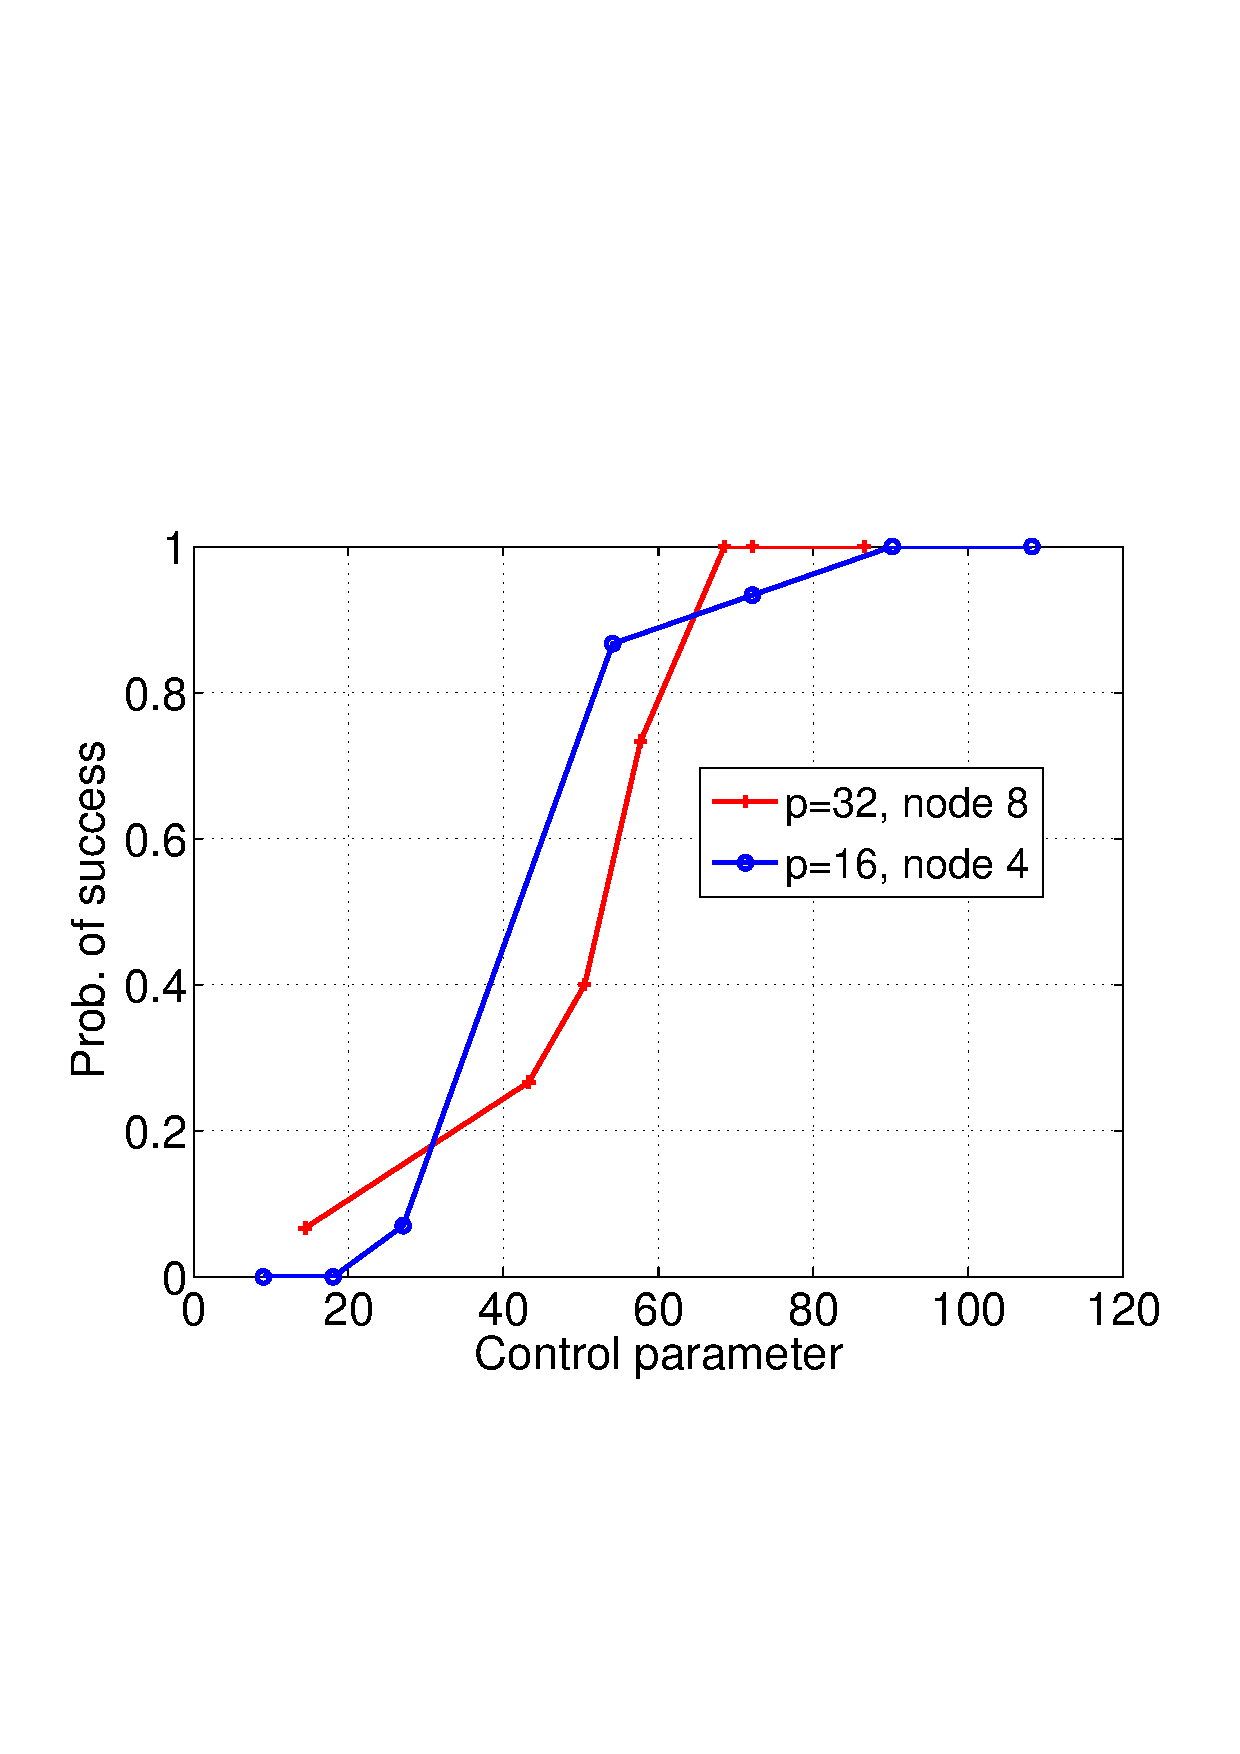
\includegraphics[scale=0.3]{figures/nbdRecovery-chain}
% \label{fig:graphtype:line}
}
\subfigure[Grid]{
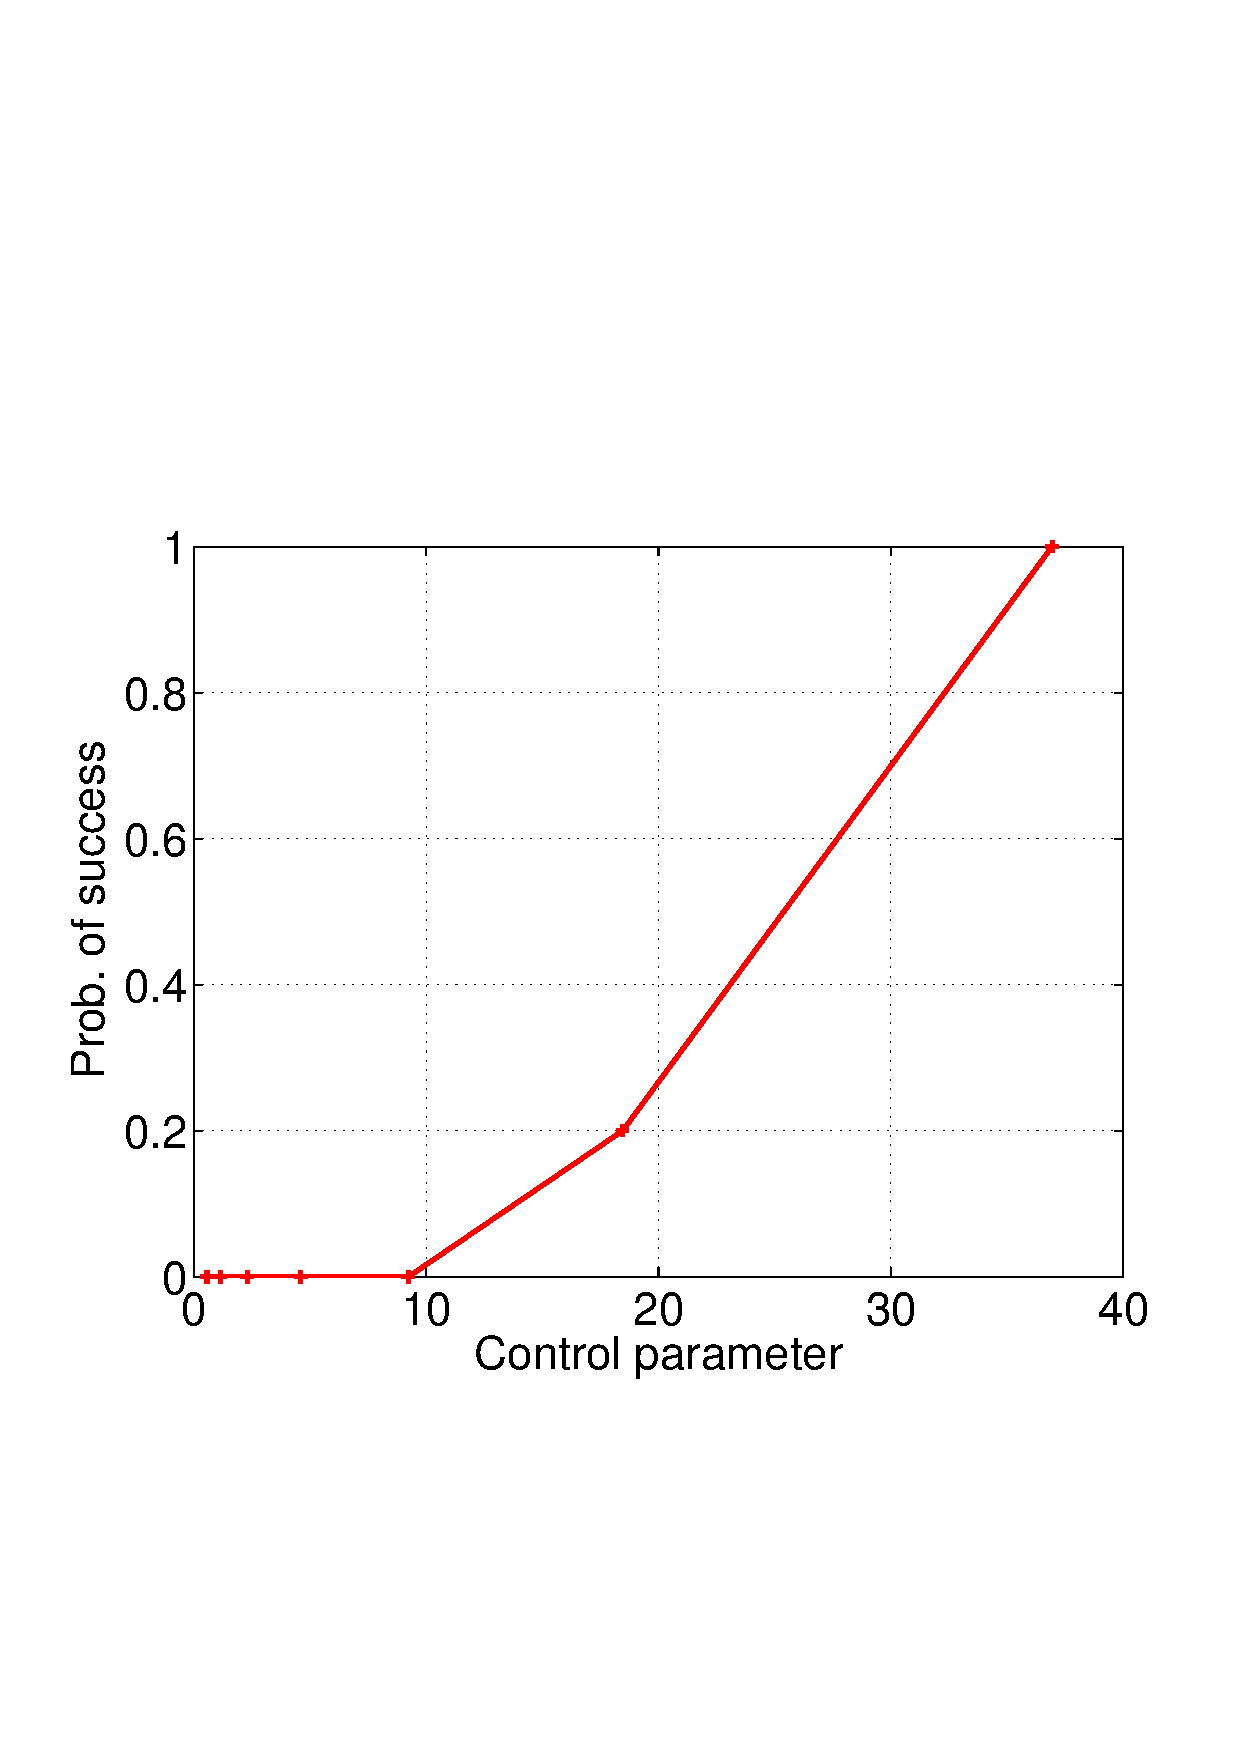
\includegraphics[scale=0.3]{figures/grid16nNode6}
% \label{fig:graphtype:grid}
}
\label{fig:neighborhoodrecovery}
\caption{Probability of success \small$\mathbb{P}[\widehat{\N}(\svert) = \N(\svert)]$\normalsize versus the control parameter $\beta(n, p, d) = \frac{n}{10 d \log(p)}$ for discrete graphical models on a Line Graph and a Grid.}
 
\end{figure}

\begin{figure}[t]
\centering
\subfigure[Line Graph]{
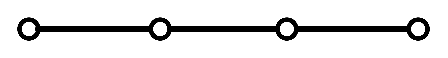
\includegraphics[scale=0.3]{Drawing1.eps}
\label{fig:graphtype:line}
}
\subfigure[Grid]{
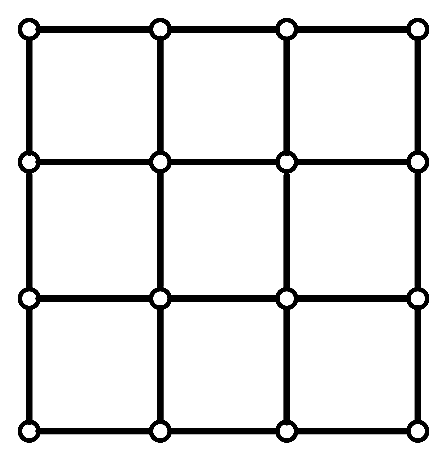
\includegraphics[scale=0.3]{Drawing2.eps}
\label{fig:graphtype:grid}
}
\subfigure[Three-Way]{
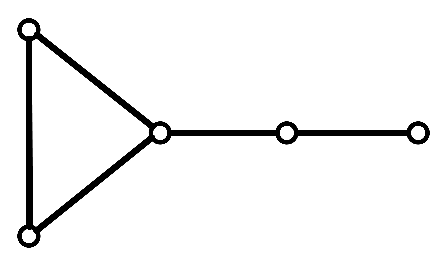
\includegraphics[scale=0.3]{Drawing3.eps}
\label{fig:graphtype:threeway}
}
\label{fig:graphtype}
\caption[Graph Types:]{Line graph \subref{fig:graphtype:line} and Grid \subref{fig:graphtype:grid} are used in studying pairwise graphical model selection. Three-way graph \subref{fig:graphtype:threeway} is used for studying higher-order graphical model selection.}
\end{figure}


\begin{figure}[t]
\centering
\includegraphics[scale=0.3]{figures/spade16nNode3.eps}
\label{fig:higherOrder}
\caption{Probability of success \small$\mathbb{P}[\widehat{\N}(\svert) = \N(\svert))]$\normalsize versus the control parameter $\beta(n, p, d) = \frac{n}{10 d \log(p)}$ for a higher order discrete graphical model on a Three-way graph.}
\end{figure}

\section{Experiments}
\noindent In this section, we report a set of synthetic experiments investigating the consequences of the main theorems. These results illustrate the behavior of the structure learning algorithm on various types of graphs. We fix the size of the alphabet $m=3$. For a given graph type, we pick a pairwise parameter set $\Theta^*$. We generate $n$ samples according to the probability distribution corresponding to $\Theta^*$. Then, we solve \eqref{EqnPairwiseGroup} and compare the graph corresponding to the solution with the original graph. If the two graphs are identical, we declare that the algorithm has succeeded.


{\bf Pairwise Model:} We consider two different classes of graphs: line graphs and grids (Fig.~\ref{fig:graphtype}). In particular, we consider line graphs of size $p=16,32$ and a grid of size $\sqrt{p}\times \sqrt{p} = 16$. In each of these cases, the parameter vector $\Theta^*$ is generated by setting each non-zero entry $\theta^*_{\svert t;jk} \in [-0.5, 0.5]$ for the line graphs and $\theta^*_{\svert t;jk} \in [0, 5]$ for the grid unfirmly at random. To estimate the probability of success, we use $15$ batches of samples drawn from the distribution specified by $\Theta^*$. We consider two types of simulations:

%\begin{itemize}

%\item 
\noindent {\bf Neighborhood Recovery:} Here, we focus on the recovery of the neighborhood of a particular node in a graph. Fixing a sample batch, for each pair $(p,n)$, we set $\regpar_n=K\left(\sqrt{\frac{p-1}{n}}+\frac{m-1}{4\sqrt{n}}\right)$, where $K$ is the constant chosen by cross validation. We compare the graph induced by $\widehat{\Theta}_{K^*}$ with the graph induced by $\Theta^*$ to get the probability of success. Fig~\ref{fig:neighborhoodrecovery} shows the probability of success in neighborhood recovery. Notice that for different values of $n$ and $p$, the phase transition graphs stack on the top of each other; this shows that the scaling of the samples $n$ is correct.

%\item {\bf Graph Recovery:} We then, investigate the recovery of the whole graph. Solving the optimization problem \eqref{EqnPairwiseGroup} for all nodes, we declare success if the recovered neighborhood of all nodes exactly matches the true neighborhood. Fig.~\ref{fig:graphrecovery} shows the probability of success in recovery of the graph structure using our method. 
%\end{itemize}


{\bf Higher-Order Model:} In this case, we consider a graph with higher order dependencies and try to estimate it using the pairwise model. We consider the three-way graph (triangle + line graph of size $p-2$) shown in Fig~\ref{fig:graphtype:threeway}. There is only one three-way factor involving three nodes. The rest of the graph is characterized by pairwise parameters. Solving \eqref{EqnGroupHigherOrder}, we investigate the probability of success for neighborhood recovery of the node that connects the line graph and the triangle. Fig.~\ref{fig:higherOrder} illustrates the result.



\newpage
\bibliography{dgm}

\newpage\phantom{.}\newpage
% \documentclass{article}
% 
% \usepackage{aistats2e}
% 
% \usepackage{epsfig, graphics}
% \usepackage{latexsym}
% \usepackage{amsmath,amsthm,amssymb,amsfonts}
% \usepackage{fullpage}
% \usepackage[numbers]{natbib}
% 
% \usepackage[T1]{fontenc}
% %\usepackage{avant}
% \renewcommand*\familydefault{\sfdefault}
% \newtheorem{definition}{Definition}
% \newtheorem{proposition}{Proposition}
% \newtheorem{theorem}{Theorem}
% \newtheorem{lemma}{Lemma}
% \newcommand{\myparagraph}[1]{\noindent \paragraph{#1}}
% \newcommand{\comment}[1]{}
% \newcommand{\tr}[2]{\left<#1,#2\right>}
% \newcommand{\matnorm}[2]{|\!|\!|#1|\!|\!|_{#2}}
% \newcommand{\norm}[2]{\left\|#1\right\|_{#2}}
% \newcommand{\flaten}[1]{\mathbf{v}\left(#1\right)}
% \def\M{\mathcal{M}}
% \def\N{\mathcal{N}}
% \def\A{\mathcal{A}}
% \def\X{\mathcal{X}}
% \def\I{\mathcal{I}}
% \def\J{\mathcal{J}}
% \def\real{\mathbb{R}}
% \def\pdim{p}
% \def\mdim{m}
% \def\kdim{k}
% \def\numobs{n}
% \def\Data{D}
% \def\regpar{\lambda}
% 
% \newenvironment{carlist}
% {\begin{list}{$\bullet$}
% {\setlength{\topsep}{0in} \setlength{\partopsep}{0in}
%  \setlength{\parsep}{0in} \setlength{\itemsep}{\parskip}
%  \setlength{\leftmargin}{0.07in} \setlength{\rightmargin}{0.08in}
%  \setlength{\listparindent}{0in} \setlength{\labelwidth}{0.08in}
%  \setlength{\labelsep}{0.1in} \setlength{\itemindent}{0in}}}
% {\end{list}}
% \def\vertex{V}
% \def\edge{E}
% \def\statenum{m}
% \def\svert{\ensuremath{r}}
% \def\defn{:=}
% \def\fisher{Q}
% \def\support{S}
% \def\dual{Z}
% 
% %\synctex=0
% \title{Learning Discrete Graphical Models}
% 
% \date{}
% 
% \begin{document}
% 
% \maketitle
% 
% 
\noindent
{\Large {\bf Supplementary Material}}


%\appendix
\section{Auxiliary Lemmas: Proof of Lemma~\ref{LemSuffOptCond}}


\begin{proof}
We can rewrite \eqref{EqnPairwiseGroup} as an optimization problem over the $\ell_1/\ell_2$ ball of radius $C$ for some $C(\regpar_n)<\infty$. Since $\lambda_n>0$, by KKT conditions, $\norm{\widetilde{\Theta}_{\backslash \svert}}{1,2}=C$ for all optimal primal solution $\widetilde{\Theta}_{\backslash \svert}$.

\noindent By definition of the $\ell_1/\ell_2$ subdifferential, we know that for any column $u\in\vertex\backslash\{\svert\}$, we have $\left\|\left(\hat{\dual}_{\backslash \svert}\right)_u\right\|_2\leq 1$. Considering the necessary optimality condition $\nabla\ell\left(\hat{\Theta}_{\backslash \svert}\right)+\regpar_n \hat{\dual}_{\backslash \svert}=0$, by complementary slackness condition, we have $\tr{\widetilde{\Theta}_{\backslash \svert}}{\hat{\dual}_{\backslash \svert}}-C=\tr{\widetilde{\Theta}_{\backslash \svert}^T}{\hat{\dual}_{\backslash \svert}}-\norm{\widetilde{\Theta}_{\backslash \svert}}{1,2}=0$. Now if for an arbitrary column $u\in\vertex\backslash\{\svert\}$, we have $\left\|\left(\hat{\dual}_{\backslash \svert}\right)_u\right\|_2<1$ and $\left(\widetilde{\Theta}_{\backslash \svert}\right)_u \neq 0$ then this would contradict the condition that $\tr{\widetilde{\Theta}_{\backslash \svert}}{\hat{\dual}_{\backslash \svert}} = \norm{\widetilde{\Theta}_{\backslash \svert}}{1,2}$.

For this restricted problem, if the Hessian sub-matrix is positive definite, then the problem is strictly convex and it has a unique solution.\\
\end{proof}



\section{Derivatives of the Log-Likelihood Function}
In this section, we point out the key properties of the gradient, Hessian and derivative of the Hessian for the log-liklihood function. These properties are used to prove the concentration lemmas.

\subsection{Gradient}
By simple derivation, we have
\begin{equation}
\begin{aligned}
&\frac{\partial}{\partial\theta^*_{\svert t;\ell k}}\ell^{(i)}(\Theta_{\backslash \svert}; \Data) \\ &\,=\! \I\left[x_t^{(i)}=k\right]\!\! \left(\!\I\left[x_\svert^{(i)}\!\!=\!\ell\right]\!\! -\! \mathbb{P}_{\Theta^*_{\backslash\svert}}\!\! \left[X_\svert\!\! =\! \ell \! \mid \! X_{\backslash \svert}\! =\!
x_{\backslash \svert}^{(i)}\right]\!\right)\!.
\end{aligned}
\nonumber
\end{equation}
It is easy to show that $\mathbb{E}_{\Theta^*_{\backslash\svert}}\!\!\left[\!\frac{\partial}{\partial\theta^*_{rt;\ell k}}\ell^{(i)}(\Theta_{\backslash \svert}; \Data)\!\right]\!=\!0$ and $\!\text{Var}\!\left(\!\frac{\partial}{\partial\theta^*_{rt;\ell k}}\ell^{(i)}(\!\Theta_{\backslash \svert}; \Data)\!\right)\!\!\leq\!\!\frac{1}{4}$. With i.i.d assumption on drawn samples, we have $\text{Var}\left(\frac{\partial}{\partial\theta^*_{rt;\ell k}}\ell(\Theta_{\backslash \svert}; \Data)\right)=\text{Var}\left(\frac{1}{n}\sum_{i=1}^n\frac{\partial}{\partial\theta^*_{rt;\ell k}}\ell^{(i)}(\Theta_{\backslash \svert}; \Data)\right)\leq\frac{1}{4n}$. Hence, for a fixed $t\in\vertex\backslash\{\svert\}$ by Jensen's inequality,
\begin{equation}
\begin{aligned}
&\mathbb{E}_{\Theta^*_{\backslash\svert}}\left[\norm{\frac{\partial}{\partial\theta^*_{\svert t;\ell k}}\ell(\Theta_{\backslash \svert}; \Data)}{2}\right]\\
&\qquad\qquad\qquad\leq\sqrt{\mathbb{E}_{\Theta^*_{\backslash\svert}}\left[\norm{\frac{\partial}{\partial\theta^*_{\svert t;\ell k}}\ell(\Theta_{\backslash \svert}; \Data)}{2}^2\right]}\\
&\qquad\qquad\qquad\leq\frac{m-1}{2\sqrt{n}}.
\end{aligned}
\nonumber
\end{equation}
Considering the terms associated with $\theta^*_{\svert t;\ell k}$'s in the gradient vector of the log-likelihood function, for a fixed $t\in\vertex\backslash\{\svert\}$, only $m-1$ (out of $(m-1)^2$) values are non-zero. By a simple calculation, we get
\begin{equation}
\max_{t\in\vertex\backslash\{\svert\}}\norm{\frac{\partial}{\partial\theta^*_{\svert t;\ell k}}\ell^{(i)}(\Theta_{\backslash \svert}; \Data)}{2}\leq\sqrt{2}\qquad\forall i.\\
\nonumber
\end{equation}
By Azuma-Hoeffding inequality, we get
\begin{equation}
\mathbb{P}\left[\norm{\frac{\partial}{\partial\theta^*_{\svert t;\ell k}}\ell(\Theta_{\backslash \svert}; \Data)}{2}\!\!\!>\!\!\frac{m-1}{2\sqrt{n}}\!+\!\epsilon\right]\!\!\leq\! 2\exp\left(\!-\frac{\epsilon^2}{4}n\!\right),
\nonumber
\end{equation}
for all $t\in\vertex\backslash\{\svert\}$. Using the union bound, we get
\begin{equation}
\begin{aligned}
&\mathbb{P}\left[\max_{t\in\vertex\backslash\{\svert\}}\norm{\frac{\partial}{\partial\theta^*_{\svert t;\ell k}}\ell(\Theta_{\backslash \svert}; \Data)}{2}\!\!\!>\!\frac{m-1}{2\sqrt{n}}\!+\!\epsilon\right] \\&\qquad\qquad\qquad\qquad\quad\leq 2\exp\left(-\frac{\epsilon^2}{4}n+\log(p-1)\right).\\
\end{aligned}
\label{gradient_inf_2_bound}
\end{equation}

\subsection{Hessian}
\label{Hessian_Section}
\noindent For the Hessian of the log-likelihood function, we have
\begin{equation}
\frac{\partial^2\, \ell^{(i)}(\Theta_{\backslash \svert}; \Data)}{\partial\theta^*_{\svert t_2;\ell_2 k_2}\, \partial\theta^*_{\svert t_1;\ell_1 k_1}}\! =\! \I\!\left[x_{t_1}^{(i)}\!\!=\!k_1\!\right] \!\!\I\!\left[x_{t_2}^{(i)}\!\!=\!k_2\!\right]\! \eta_{\ell_1\ell_2}\!\!\left(\!x^{(i)}\!\right)\!\!,
\nonumber 
\end{equation}
where,
\begin{equation}
\begin{aligned}
&\eta_{\ell_1\ell_2}\left(x^{(i)}\right) \defn \mathbb{P}_{\Theta^*_{\backslash\svert}} \left[X_\svert = \ell_1 \, \Big| X_{\backslash \svert} =
x_{\backslash \svert}^{(i)}\right] \\ &\left(\!\!\I\left[x_\svert^{(i)}\!\!=\!\ell_1\right]\!\I\left[x_\svert^{(i)}\!\!=\!\ell_2\right] \!-\! \mathbb{P}_{\Theta^*_{\backslash\svert}} \left[X_\svert \!\!=\! \ell_2 \! \Big| X_{\backslash \svert}\! =\!
x_{\backslash \svert}^{(i)}\right]\!\right).\\
\end{aligned}
\nonumber
\end{equation}

\noindent Consider the zero-mean random variable
\begin{equation}
\begin{aligned}
&Z^{(i)}_{t_1\ell_1k_1;t_2\ell_2k_2}:=\\
&\qquad\frac{\partial^2\, \ell^{(i)}(\Theta_{\backslash \svert}; \Data)}{\partial\theta^*_{\svert t_2;\ell_2 k_2}\, \partial\theta^*_{\svert t_1;\ell_1 k_1}}-\mathbb{E}\left[\frac{\partial^2\, \ell(\Theta_{\backslash \svert}; \Data)}{\partial\theta^*_{\svert t_2;\ell_2 k_2}\, \partial\theta^*_{\svert t_1;\ell_1 k_1}}\right].
\end{aligned}
\nonumber
\end{equation}
\noindent Notice that $\text{Var}\left(Z^{(i)}_{t_1\ell_1k_1;t_2\ell_2k_2}\right)\leq 1$ and consequently, by i.i.d assumption, $\text{Var}\left(\frac{1}{n}\sum_{i=1}^nZ^{(i)}_{t_1\ell_1k_1;t_2\ell_2k_2}\right)\leq \frac{1}{n}$. Hence, for fixed values $t_1,\ell_1,k_1$ and $t_2\in\support_2\subseteq\vertex\backslash\{\svert\}$, we have
\begin{equation}
\begin{aligned}
&\mathbb{E}_{\Theta^*_{\backslash\svert}}\left[\norm{\frac{1}{n}\sum_{i=1}^nZ^{(i)}_{t_1\ell_1k_1;t_2\ell_2k_2}}{2}\right]\\
&\qquad\qquad\qquad\leq\sqrt{\mathbb{E}_{\Theta^*_{\backslash\svert}}\left[\norm{\frac{1}{n}\sum_{i=1}^nZ^{(i)}_{t_1\ell_1k_1;t_2\ell_2k_2}}{2}^2\right]}\\
&\qquad\qquad\qquad\leq\sqrt{\frac{|S_2|}{n}}.
\end{aligned}
\label{eq1}
\end{equation}
This radom variable, for fixed values $t_1,\ell_1,k_1$ and a fixed $t_2$, is bounded and in particular, $\norm{\frac{1}{n}\sum_{i=1}^nZ^{(i)}_{t_1\ell_1k_1;t_2\ell_2k_2}}{2}\leq 2$. By Azuma-Hoeffding inequality and the union bound,
\begin{equation}
\begin{aligned}
&\mathbb{P}\left[\norm{\fisher^n_{\support_\svert\support_\svert} -\fisher^*_{\support_\svert\support_\svert}}{\infty,2}>\frac{\sqrt{d_\svert}}{\sqrt{n}}+\epsilon\right]\\
&\qquad\qquad\qquad\leq 2\exp\left(-\frac{\epsilon^2}{8}n+\log\left((m-1)^2d_\svert\right)\right).\\
&\mathbb{P}\left[\norm{\fisher^n_{\support_\svert^c\support_\svert} -\fisher^*_{\support_\svert^c\support_\svert}}{\infty,2}>\frac{\sqrt{d_\svert}}{\sqrt{n}}+\epsilon\right]\\
&\qquad\leq 2\exp\left(-\frac{\epsilon^2}{8}n+\log\left((m-1)^2(p\!-\!d_\svert\!-\!1)\right)\right)\!.\\
\end{aligned}
\label{fisher_inf_1_bound1}
\end{equation}
Similar analysis as \eqref{eq1} combined with the ineqality $\Lambda_{\max}(\cdot)\leq\norm{\cdot}{\infty,2}$, shows that
\begin{equation}
\begin{aligned}
&\mathbb{P}\left[\Lambda_{\max}\left(\fisher^n_{\support_\svert\support_\svert} -\fisher^*_{\support_\svert\support_\svert}\right)>\frac{\sqrt{d_\svert}}{\sqrt{n}}+\epsilon\right]\\ &\qquad\qquad\qquad\leq\, 2\exp\left(-\frac{\epsilon^2}{8}n+\log\left((m-1)^2d_\svert\right)\!\right)\!.\\
\end{aligned}
\label{fisher_2_bound}
\end{equation}
We also need a control over the deviation of the inverse sample Fisher information matrix from the inverse of its mean. We have
\begin{equation}
\begin{aligned}
&\Lambda_{\max}\left(\left(\fisher^n_{\support_\svert\support_\svert}\right)^{-1} -\left(\fisher^*_{\support_\svert\support_\svert}\right)^{-1}\right)\\ &\,=\Lambda_{\max}\left(\left(\fisher^*_{\support_\svert\support_\svert}\right)^{-1} \left(\fisher^*_{\support_\svert\support_\svert} -\fisher^n_{\support_\svert\support_\svert}\right) \left(\fisher^n_{\support_\svert\support_\svert}\right)^{-1}\right)\\
&\,\leq\Lambda_{\max}\left(\left(\fisher^*_{\support_\svert\support_\svert}\right)^{-1}\right)
\Lambda_{\max}\left(\fisher^*_{\support_\svert\support_\svert} -\fisher^n_{\support_\svert\support_\svert}\right)\\ &\qquad\qquad\qquad\qquad\qquad\qquad\qquad\Lambda_{\max}\left(\left(\fisher^n_{\support_\svert\support_\svert}\right)^{-1}\right)\\
&\,\leq\frac{\sqrt{d_\svert}}{C_{\min}\sqrt{n}} \Lambda_{\max}\left(\left(\fisher^n_{\support_\svert\support_\svert}\right)^{-1}\right).\\
\end{aligned}
\nonumber
\end{equation}
By part (B1) in Lemma~\ref{Concentration_Lemma}, we have
\begin{equation}
\begin{aligned}
&\mathbb{P}\left[\Lambda_{\max}\left(\left(\fisher^n_{\support_\svert\support_\svert}\right)^{-1}\right) >\frac{1}{C_{\min}}+\epsilon\right]\\ &\,\leq \! 2\exp\left(\!\!-\frac{\left(\frac{C_{\min}\epsilon\sqrt{n}\!\!}{1+C_{\min}\epsilon}-\sqrt{d_\svert}\right)^2}{8}+\!\log\left((m-1)^2d_\svert\right)\!\right)\!.
\end{aligned}
\label{sample_fisher_2_bound}
\end{equation}
Hence, we get,
\begin{equation}
\begin{aligned}
&\mathbb{P}\left[\Lambda_{\max}\left(\left(\fisher^n_{\support_\svert\support_\svert}\right)^{-1}\!\!\!\!\! -\!\left(\fisher^*_{\support_\svert\support_\svert}\right)^{-1}\right) >\frac{\sqrt{d_\svert}}{C_{\min}^2\sqrt{n}}\!+\!\epsilon\right]\\
&\,\leq\! 4\exp\left(\!\!-\frac{\left(\frac{C_{\min}\epsilon\sqrt{n}\!\!}{1+C_{\min}\epsilon}-\sqrt{d_\svert}\right)^2}{8}+\!\log\left((m-1)^2d_\svert\right)\!\right)\!.
\end{aligned}
\label{fisher_inf_1_bound2}
\end{equation}

\subsection{Derivative of Hessian}
\label{derivative_hessian}
We want to bound the rate of the change for the elements of Hessian matrix. Let
\begin{equation}
\begin{aligned}
&\nabla\fisher_{t_2\ell_2k_2;t_1\ell_1k_1}^{(i)}\\
&\qquad:= \frac{\partial}{\partial\Theta_{\backslash\svert}}\frac{\partial^2\, \ell^{(i)}(\Theta_{\backslash \svert}; \Data)}{\partial\theta^*_{\svert t_2;\ell_2 k_2}\, \partial\theta^*_{\svert t_1;\ell_1 k_1}}\\
&\qquad=\I\left[x_{t_1}^{(i)}=k_1\right] \I\left[x_{t_2}^{(i)}=k_2\right] \frac{\partial}{\partial\Theta_{\backslash\svert}}\eta_{\ell_1\ell_2}\left(x^{(i)}\right).
\end{aligned}
\nonumber
\end{equation}
Recall the definition of $\eta(\cdot)$ from section~\ref{Hessian_Section}. We have
\begin{equation}
\begin{aligned}
&\frac{\partial\eta_{\ell_1\ell_2}\left(x^{(i)}\right)}{\partial\theta_{\svert t_3;\ell_3k_3}}\! =\! \I\left[x_{t_3}^{(i)}\!\!=\!k_3\right] \mathbb{P}_{\Theta^*_{\backslash\svert}}\!\! \left[X_\svert\!\! =\! \ell_1 \! \Big| X_{\backslash \svert}\! =\!
x_{\backslash \svert}^{(i)}\right]\\ &\qquad\left(\eta_{\ell_2\ell_3}\left(x^{(i)}\right)-\frac{\eta_{\ell_1\ell_2}\left(x^{(i)}\right) \eta_{\ell_1\ell_3}\left(x^{(i)}\right)} {\mathbb{P}_{\Theta^*_{\backslash\svert}} \left[X_\svert = \ell_1 \, \Big| X_{\backslash \svert} =
x_{\backslash \svert}^{(i)}\right]^2}\right).
\end{aligned}
\nonumber
\end{equation}
For any $t_3\in\vertex\backslash\{\svert\}$, each entry is bounded by $\frac{1}{2}$ and there are only $m-1$ non-zero entries for each $k_3$. Hence, for any $t_3$, one can colculde that $\norm{\frac{\partial}{\partial\theta_{\svert t_3;\ell_3k_3}}\eta_{\ell_1\ell_2}\left(x^{(i)}\right)}{2}\leq\frac{m-1}{\sqrt{2}}$ for all $i$. Finally, for all $\ell_1$ and $\ell_2$ we have
\begin{equation}
\max_{t_3\in\vertex\backslash\{\svert\}} \norm{\frac{\partial}{\partial\theta_{\svert t_3;\ell_3k_3}}\eta_{\ell_1\ell_2}\left(x^{(i)}\right)}{2}\leq\frac{m-1}{\sqrt{2}}.
\label{derivative_hessian_eq}
\end{equation}


\section{Proof of Lemma~\ref{Concentration_Lemma}}
\noindent {\bf (B1)} By variational representation of the smallest eigenvalue, we have
\begin{equation}
\begin{aligned}
\Lambda_{\min}\left(\fisher^*_{\support_\svert\support_\svert}\right) &= \min_{\norm{x}{2}=1}x^T\fisher^*_{\support_\svert\support_\svert}x\\
&\leq y^T\fisher^n_{\support_\svert\support_\svert}y + y^T\left(\fisher^*_{\support_\svert\support_\svert}-\fisher^n_{\support_\svert\support_\svert}\right)y,
\end{aligned}
\nonumber
\end{equation}
for all $y\in\mathbb{R}^{(m-1)^2d_\svert}$ with $\norm{y}{2}=1$ and in particular for the unit-norm minimal eigenvalue of $\fisher^n_{\support_\svert\support_\svert}$. Hence,
\begin{equation}
\Lambda_{\min}\left(\fisher^n_{\support_\svert\support_\svert}\right) \!\geq\Lambda_{\min}\left(\fisher^*_{\support_\svert\support_\svert}\right) \!-\Lambda_{\max}\left(\fisher^*_{\support_\svert\support_\svert}\!\!-\!\fisher^n_{\support_\svert\support_\svert}\right).
\nonumber
\end{equation}
By \eqref{fisher_2_bound}, we get
\begin{equation}
\begin{aligned}
&\mathbb{P}\left[\Lambda_{\min}\left(\fisher^n_{\support_\svert\support_\svert}\right)< C_{\min}-\epsilon\right]\\ &\qquad\leq\mathbb{P}\left[\Lambda_{\max}\left(\fisher^*_{\support_\svert\support_\svert}-\fisher^n_{\support_\svert\support_\svert}\right) > \epsilon\right]\\ &\qquad\leq 2\exp\left(-\frac{(\epsilon\sqrt{n}-\sqrt{d_\svert})^2}{8}+\log\big((m-1)^2d_\svert\big)\right).\\
\end{aligned}
\nonumber
\end{equation}

\noindent {\bf (B2)} We can write
\begin{equation}
\begin{aligned}
&\fisher^n_{\support^c_\svert\support_\svert}\left(\fisher^n_{\support_\svert\support_\svert}\right)^{-1}= \underbrace{\fisher^*_{\support^c_\svert\support_\svert}\left(\fisher^*_{\support_\svert\support_\svert}\right)^{-1}}_{T_0}\\
&\qquad+\underbrace{\fisher^*_{\support^c_\svert\support_\svert} \left(\left(\fisher^n_{\support_\svert\support_\svert}\right)^{-1} -\left(\fisher^*_{\support_\svert\support_\svert}\right)^{-1}\right)}_{T_1}\\
&\qquad+\underbrace{\left(\fisher^n_{\support^c_\svert\support_\svert}-\fisher^*_{\support^c_\svert\support_\svert}\right) \left(\fisher^*_{\support_\svert\support_\svert}\right)^{-1}}_{T_2}\\
&\qquad+\underbrace{\left(\fisher^n_{\support^c_\svert\support_\svert}-\fisher^*_{\support^c_\svert\support_\svert}\right) \left(\left(\fisher^n_{\support_\svert\support_\svert}\right)^{-1}\!\!\!\! -\left(\fisher^*_{\support_\svert\support_\svert}\right)^{-1}\right)}_{T_3}.\\
\end{aligned}
\nonumber
\end{equation}
Considering assumption (A3), $\norm{T_0}{\infty,2}<\frac{1-2\alpha}{\sqrt{d_\svert}}$ and hence, it suffices to show that $\norm{T_i}{\infty,2}<\frac{\alpha}{3\sqrt{d_\svert}}$ for $i=1,2,3$. For the first term, we have
\begin{equation}
\begin{aligned}
&\norm{\fisher^*_{\support^c_\svert\support_\svert} \left(\left(\fisher^n_{\support_\svert\support_\svert}\right)^{-1}\!\!\!\! -\left(\fisher^*_{\support_\svert\support_\svert}\right)^{-1}\right)}{\infty,2}\\ &\,=\!\!\norm{\fisher^*_{\support^c_\svert\support_\svert} \left(\fisher^*_{\support_\svert\support_\svert}\right)^{-1}\!\! \left(\fisher^*_{\support_\svert\support_\svert}\!\! -\!\fisher^n_{\support_\svert\support_\svert}\right) \left(\fisher^n_{\support_\svert\support_\svert}\right)^{-1}}{\infty,2}\\
&\,\leq\!\!\norm{\fisher^*_{\support^c_\svert\support_\svert} \left(\fisher^*_{\support_\svert\support_\svert}\right)^{-1}}{\infty,2} \Lambda_{\max}\left(\fisher^*_{\support_\svert\support_\svert} -\fisher^n_{\support_\svert\support_\svert}\right)\\ &\qquad\qquad\qquad\qquad\qquad\qquad\qquad\Lambda_{\max}\left(\left(\fisher^n_{\support_\svert\support_\svert}\right)^{-1}\right)\\
&\,\leq\frac{1-2\alpha}{\sqrt{d_\svert}}\frac{\sqrt{d_\svert}}{\sqrt{n}}\frac{1}{C_{\min}}.
\end{aligned}
\nonumber
\end{equation}
The last inequality follows from \eqref{fisher_inf_1_bound1} and \eqref{sample_fisher_2_bound} with high probability. Setting $\bar{C}_{\min}=\min\left(C_{\min},1\right)$, by applying the union bound,
\begin{equation}
\begin{aligned}
&\mathbb{P}\left[\norm{\fisher^*_{\support^c_\svert\support_\svert} \left(\left(\fisher^n_{\support_\svert\support_\svert}\right)^{-1} -\left(\fisher^*_{\support_\svert\support_\svert}\right)^{-1}\right)}{\infty,2}>\epsilon\right]\\
&\leq\! 4\!\exp\!\left(\!\!-\frac{\left(\bar{C}_{\min}\epsilon\sqrt{n}\!-\!\sqrt{d_\svert}\!-\!\frac{1\!-2\alpha}{C_{\min}}\right)^{\!2}}{8}\!+\!\log\!\left(\!(\!m\!-\!1\!)^2\!d_\svert\!\right)\!\!\!\right)\!\!.
\end{aligned}
\nonumber
\end{equation}

For the second term, we have
\begin{equation}
\begin{aligned}
&\norm{\left(\fisher^n_{\support^c_\svert\support_\svert}-\fisher^*_{\support^c_\svert\support_\svert}\right) \left(\fisher^*_{\support_\svert\support_\svert}\right)^{-1}}{\infty,2}\\ &\qquad\qquad\leq \norm{\fisher^n_{\support^c_\svert\support_\svert}-\fisher^*_{\support^c_\svert\support_\svert}}{\infty,2} \Lambda_{\max}\left(\left(\fisher^*_{\support_\svert\support_\svert}\right)^{-1}\right)\\
&\qquad\qquad\leq\frac{\sqrt{d_\svert}}{\sqrt{n}}\frac{1}{C_{\min}}.
\end{aligned}
\nonumber
\end{equation}
The last inequality follows from \eqref{fisher_inf_1_bound1} with high probability. Hence, we have
\begin{equation}
\begin{aligned}
&\mathbb{P}\left[\norm{\left(\fisher^n_{\support^c_\svert\support_\svert} -\fisher^*_{\support^c_\svert\support_\svert}\right) \left(\fisher^*_{\support_\svert\support_\svert}\right)^{-1}}{\infty,2}>\epsilon\right]\\ &\!\leq\! 2\!\exp\!\left(\!\!-\frac{\left(\!\epsilon\sqrt{n}\!-\!\frac{\left(1\!+\!C_{\min}\right)\sqrt{d_\svert}}{C_{\min}}\!\right)^{\!2}\!\!}{8}\!+\!\log\!\left(\!(\!m\!-\!1\!)^{\!2}\!(\!p\!-\!1\!\!-\!d_\svert\!)\!\right)\!\!\!\right)\!\!.
\end{aligned}
\nonumber
\end{equation}

For the third term, we have
\begin{equation}
\begin{aligned}
&\norm{\left(\fisher^n_{\support^c_\svert\support_\svert}-\fisher^*_{\support^c_\svert\support_\svert}\right) \left(\left(\fisher^n_{\support_\svert\support_\svert}\right)^{-1}\!\!\!\! -\left(\fisher^*_{\support_\svert\support_\svert}\right)^{-1}\right)}{\infty,2}\\ &\leq\!\! \norm{\fisher^n_{\support^c_\svert\support_\svert}\!\!-\fisher^*_{\support^c_\svert\support_\svert}}{\infty,2} \!\!\Lambda_{\max}\left(\left(\fisher^n_{\support_\svert\support_\svert}\right)^{-1}\!\!\!\! -\left(\fisher^*_{\support_\svert\support_\svert}\right)^{-1}\right)\\
&\leq\frac{\sqrt{d_\svert}}{\sqrt{n}}\frac{\sqrt{d_\svert}}{C_{\min}^2\sqrt{n}}\,\,=\frac{d_\svert}{C_{\min}^2n}
\end{aligned}
\nonumber
\end{equation}
The last inequality follows from \eqref{fisher_inf_1_bound1} and \eqref{fisher_inf_1_bound2}. Hence, we have
\begin{equation}
\begin{aligned}
&\mathbb{P}\left[\norm{\left(\fisher^n_{\support^c_\svert\support_\svert}\!\! -\fisher^*_{\support^c_\svert\support_\svert}\!\right)\! \left(\!\!\left(\fisher^n_{\support_\svert\support_\svert}\right)^{\!-1}\!\!\!\! -\left(\fisher^*_{\support_\svert\support_\svert}\right)^{\!-1}\right)}{\infty,2}\!\!\!\!>\!\epsilon\right]\\ &\leq 6\exp\Biggr(-\frac{\left(\bar{C}_{\min}\epsilon\sqrt{n}-\left(1+\frac{\sqrt{d_\svert}}{C_{\min}^2\sqrt{n}}\right)\sqrt{d_\svert}\right)^2}{8}\\ &\qquad\qquad\qquad\qquad\qquad+\log\left((m-1)^2(p-1-d_\svert)\right)\Biggr).
\end{aligned}
\nonumber
\end{equation}
The result follows by substituting $\epsilon$ with $\frac{\alpha}{3\sqrt{d_\svert}}$.

\noindent {\bf (B3)} We can write
\begin{equation}
\begin{aligned}
&\mathbb{P}\left[\Lambda_{\max}\left(\J^n\right)> D_{\max}+\epsilon\right]\\ &\qquad\qquad\qquad\quad\leq\mathbb{P}\left[\norm{\frac{1}{n}\sum_{i=1}^n\left(\J^{(i)}-\J^*\right)}{F}>\epsilon\right].
\end{aligned}
\nonumber
\end{equation}
Consequently, same analysis as part (B1) gives the result.\\

This concludes the proof of the Lemma.

\section{Sufficiency Lemmas for Pairwise Dependencies}
\begin{lemma}
The constructed candidate primal-dual pair $\left(\hat{\Theta}_{\backslash \svert},\hat{\dual}_{\backslash \svert}\right)$ satisfy the conditions of the Lemma~\ref{SuffOptCond} with probability $1-c_1\exp(-c_2n)$ for some positive constants $c_1,c_2\in\mathbb{R}$.
\label{OptCertificate}
\end{lemma}

\begin{proof}
Using the mean-value theorem, for some $\bar{\Theta}_{\backslash\svert}$ in the convex combination of $\hat{\Theta}_{\backslash\svert}$ and $\Theta^*_{\backslash\svert}$, we have
\begin{equation}
\begin{aligned}
&\nabla^2\ell\left(\Theta^*_{\backslash\svert};D\right)\left[\hat{\Theta}_{\backslash\svert}-\Theta^*_{\backslash\svert}\right]\\ &=\nabla\ell\left(\hat{\Theta}_{\backslash\svert};D\right)-\nabla\ell\left(\Theta^*_{\backslash\svert};D\right)\\ &\quad+\left(\nabla^2\ell\left(\Theta^*_{\backslash\svert};D\right)-\nabla^2\ell\left(\bar{\Theta}_{\backslash\svert};D\right)\right)\left[\hat{\Theta}_{\backslash\svert}-\Theta^*_{\backslash\svert}\right]\\
&=-\regpar_n\hat{\dual}_{\backslash\svert}-\underbrace{\nabla\ell\left(\Theta^*_{\backslash\svert};D\right)}_{W_{\backslash\svert}^n}\\ &\quad+\underbrace{\left(\nabla^2\ell\left(\Theta^*_{\backslash\svert};D\right)-\nabla^2\ell\left(\bar{\Theta}_{\backslash\svert};D\right)\right) \left[\hat{\Theta}_{\backslash\svert}-\Theta^*_{\backslash\svert}\right]}_{R_{\backslash\svert}^n}.\\
\end{aligned}
\nonumber
\end{equation}
We can rewrite these set of equations as two sets of equations over $\support_\svert$ and $\support_\svert^c$. By Lemma~\ref{Concentration_Lemma}, the Hessian sub-matrix on $\support_\svert$ is invertible with high probability and thus we get
\begin{equation}
\begin{aligned}
&\fisher^n_{\support_\svert^c\support_\svert} \!\left(\fisher^n_{\support_\svert\support_\svert}\right)^{\!-1}\!\! \left(\!-\!\regpar_n\!\left(\!\hat{\dual}_{\backslash\svert}\!\right)_{\support_\svert} \!\!-\!\left(\!W_{\backslash\svert}^n\!\right)_{\support_\svert} \!\!+\!\left(\!R_{\backslash\svert}^n\!\right)_{\support_\svert}\!\right)\\ &\qquad\qquad=-\regpar_n\left(\hat{\dual}_{\backslash\svert}\right)_{\support_\svert^c} -\left(W_{\backslash\svert}^n\right)_{\support_\svert^c} +\left(R_{\backslash\svert}^n\right)_{\support_\svert^c}.
\end{aligned}
\nonumber
\end{equation}
Equivalently, we get
\begin{equation}
\begin{aligned}
\left(\hat{\dual}_{\backslash\svert}\right)_{\support_\svert^c} &= \frac{1}{\regpar_n}\left[\left(W_{\backslash\svert}^n\right)_{\support_\svert^c} \!\!\!\!-\left(R_{\backslash\svert}^n\right)_{\support_\svert^c}\right]\\ &\quad-\frac{1}{\regpar_n}\fisher^n_{\support_\svert^c\support_\svert}\! \left(\!\fisher^n_{\support_\svert\support_\svert}\right)^{\!-1} \!\!\left(\!\left(\!W_{\backslash\svert}^n\!\right)_{\support_\svert} \!\!\!\!-\left(\!R_{\backslash\svert}^n\!\right)_{\support_\svert}\!\right)\\ &\quad+\fisher^n_{\support_\svert^c\support_\svert} \left(\fisher^n_{\support_\svert\support_\svert}\right)^{-1} \left(\hat{\dual}_{\backslash\svert}\right)_{\support_\svert}.\\
\end{aligned} 
\nonumber
\end{equation}
Notice that $\norm{\left(\hat{\dual}_{\backslash\svert}\right)_{\support_\svert}}{\infty,2}=1$. Thus, we can establish the following bound
\begin{equation}
\begin{aligned}
&\norm{\left(\hat{\dual}_{\backslash\svert}\right)_{\support_\svert^c}}{\infty,2}\\ &\qquad\qquad\leq \left(1+\norm{\fisher^n_{\support_\svert^c\support_\svert} \left(\fisher^n_{\support_\svert\support_\svert}\right)^{-1}}{\infty,2}\!\!\sqrt{d_\svert}\right)\\ &\qquad\qquad\qquad\quad\left[\frac{\norm{W_{\backslash\svert}^n}{\infty,2}}{\regpar_n} +\frac{\norm{R_{\backslash\svert}^n}{\infty,2}}{\regpar_n}+1\right]-1\\
&\qquad\qquad\leq(2-\alpha)\left(\frac{\alpha}{4(2-\alpha)}+\frac{\alpha}{4(2-\alpha)}+1\right)-1\\ &\qquad\qquad= 1-\frac{\alpha}{2} \,<\, 1.
\end{aligned}
\nonumber
\end{equation}
The second inequality holds with high probability acoording to Lemma~\ref{Concentration_Lemma} and Lemma~\ref{generalbounds}.\\
\end{proof}

\begin{lemma}
For quantities defined in the proof of Lemma~\ref{OptCertificate}, the following inequalities hold:
\begin{equation}
\begin{aligned}
&\mathbb{P}\left[\frac{\norm{W_{\backslash\svert}^n}{\infty,2}}{\lambda_n} \geq \frac{\alpha}{4(2-\alpha)}\right]\\ &\quad\leq 2\exp\left(-\frac{\left(\frac{\alpha}{4(2-\alpha)}\regpar_n\sqrt{n} - \frac{m-1}{2}\right)^2}{4}+\log(p-1)\right)\\
&\mathbb{P}\left[\frac{\norm{R_{\backslash\svert}^n}{\infty,2}}{\regpar_n}>\frac{\alpha}{4(2-\alpha)}\right]\\ &\quad\leq 2\exp\left(-\frac{\left(\frac{\alpha}{4(2-\alpha)}\regpar_n\sqrt{n} - \frac{m-1}{2}\right)^2}{4}+\log(p-1)\right)\!\!.\\
\end{aligned}
\nonumber
\end{equation}
\label{generalbounds}
\end{lemma}

\begin{proof}
The first inequality follows directly from \eqref{gradient_inf_2_bound}, for $\epsilon=\frac{\alpha}{4(2-\alpha)}\regpar_n-\frac{m-1}{2\sqrt{n}}$, provided that $\regpar_n\geq\frac{2(2-\alpha)}{\alpha}\frac{m-1}{\sqrt{n}}$. This probability goes to zero, if $\regpar_n\geq\frac{8(2-\alpha)}{\alpha}\left(\sqrt{\frac{\log(p-1)}{n}}+\frac{m-1}{4\sqrt{n}}\right)$.\\

\noindent Before we proceed, we want to point out a technical fact that we will use it through the rest of the proof. For $\regpar_n$ achieves the lower bound mentioned above, any positive value $K$ and $n\geq\frac{1}{K^2}\frac{64(2-\alpha)^2}{\alpha^2}\left(\sqrt{\log(p-1)}+\frac{m-1}{4}\right)^2d_\svert^{\,2}$, we have $\regpar_nd_\svert\leq K$. Hence, we can assume $\regpar_nd_\svert$ is less than any \emph{fixed} constant $K$ for sufficiently large $n$.\\

\noindent In order to bound $R^n_{\backslash\svert}$, we need to bound \footnotesize $\norm{\left(\hat{\Theta}_{\backslash\svert}\right)_{\support_\svert}-\left(\Theta^*_{\backslash\svert}\right)_{\support_\svert}}{\infty,2}$\normalsize, using the technique used in \citet{Rothman08}. Let $G:\mathbb{R}^{(m-1)^2d_\svert}\rightarrow\mathbb{R}$ be a function defined as\footnotesize
\begin{equation}
\begin{aligned}
G\Big(\left(U\right)_{\support_\svert}\Big) &:=\ell\left(\left(\Theta^*_{\backslash\svert}\right)_{\support_\svert}\!\!+\!\left(U\right)_{\support_\svert};D\right) \!-\!\ell\left(\left(\Theta^*_{\backslash\svert}\right)_{\support_\svert};D\right)\\ &\quad+\!\regpar_n\left(\!\norm{\!\left(\Theta^*_{\backslash\svert}\right)_{\support_\svert} \!+\!\left(U\right)_{\support_\svert}}{1,2} \!\!\!\!\!-\!\norm{\!\left(\Theta^*_{\backslash\svert}\right)_{\support_\svert}}{1,2}\right).
\end{aligned}
\nonumber
\end{equation}\normalsize
By optimality of $\hat{\Theta}_{\backslash\svert}$, it is clear that \footnotesize $\left(\hat{U}\right)_{\support_\svert} =\left(\hat{\Theta}_{\backslash\svert}\right)_{\support_\svert} -\left(\Theta^*_{\backslash\svert}\right)_{\support_\svert}$\normalsize minimizes $G$. Since $G(\mathbf{0})=0$ by construction, we have \footnotesize$G\Big(\left(\hat{U}\right)_{\support_\svert}\Big)\leq 0$\normalsize. Suppose there exist an $\ell_\infty/\ell_2$ ball with radius $B_\svert$ such that for any \footnotesize$\norm{\left(U\right)_{\support_\svert}}{\infty,2}=B_\svert$\normalsize, we have that $G\Big(\left(U\right)_{\support_\svert}\Big)>0$. Then, we can claim that $\norm{\left(\hat{U}\right)_{\support_\svert}}{\infty,2}\leq B_\svert$; because if, in contrary, we assume that \footnotesize$\left(\hat{U}\right)_{\support_\svert}$\normalsize is outside the ball, then for an appropriate choice of $t\in(0,1)$, the point $t\left(\hat{U}\right)_{\support_\svert}\!\!\!+(1-t)\mathbf{0}\,\,\,$ lies on the boundary of the ball. By convexity of $G$, we have
\begin{equation}
\begin{aligned}
G\left(t\left(\hat{U}\right)_{\support_\svert}\!\!\!\!+(1-t)\mathbf{0}\right)&\!\leq t\,G\left(\!\left(\hat{U}\right)_{\support_\svert}\!\right)\!+\!(1-t)G\left(\mathbf{0}\right)\\ &\leq 0.
\end{aligned}
\nonumber
\end{equation}
This is a contradiction to the assumption of the positivity of $G$ on the boundary of the ball.\\

\noindent Let $\left(U\right)_{\support\svert}\in\mathbb{R}^{(m-1)^2d_\svert}$ be an arbitrary vector with \footnotesize$\norm{\left(U\right)_{\support_\svert}}{\infty,2}=\frac{5}{C_{\min}}\regpar_n$\normalsize.  Applying mean value theorem to the log liklihood function, for some $\beta\in[0,1]$, we get
\begin{equation}
\begin{aligned}
&G\Big(\!\left(U\right)_{\support_\svert}\!\Big) =\tr{\left(W_{\backslash\svert}\right)_{\support_\svert}} {\left(U\right)_{\support_\svert}}\\ &\quad+ \tr{\left(U\right)_{\support_\svert}}{\nabla^2\ell\left(\left(\Theta^*_{\backslash\svert}\right)_{\support_\svert}+\beta\left(U\right)_{\support_\svert};D\right) \left(U\right)_{\support_\svert}} \\ &\quad+\regpar_n\left(\norm{\left(\Theta^*_{\backslash\svert}\right)_{\support_\svert}+\left(U\right)_{\support_\svert}}{1,2} -\norm{\left(\Theta^*_{\backslash\svert}\right)_{\support_\svert}}{1,2}\right).
\end{aligned}
\label{Gu_Eqn}
\end{equation}
We bound each of these three terms individually. By Cauchy-Schwartz inequality, we have
\begin{equation}
\begin{aligned}
\left|\tr{\left(W_{\backslash\svert}\right)_{\support_\svert}} {\left(U\right)_{\support_\svert}}\right| &\leq\norm{\left(W_{\backslash\svert}\right)_{\support_\svert}}{\infty,2} \norm{\left(U\right)_{\support_\svert}}{1,2}\\
&\leq\frac{\alpha}{4(2-\alpha)}\regpar_n d_\svert \frac{5}{C_{\min}}\regpar_n\\
&\leq\frac{5}{4C_{\min}} d_\svert \regpar_n^2.
\end{aligned}
\nonumber
\end{equation}
Moreover, by triangle inequality,
\begin{equation}
\begin{aligned}
&\regpar_n\left(\norm{\left(\Theta^*_{\backslash\svert}\right)_{\support_\svert}+\left(U\right)_{\support_\svert}}{1,2} -\norm{\left(\Theta^*_{\backslash\svert}\right)_{\support_\svert}}{1,2}\right)\\ &\qquad\qquad\qquad\qquad\qquad\qquad\qquad\geq -\regpar_n \norm{\left(U\right)_{\support_\svert}}{1,2}\\
&\qquad\qquad\qquad\qquad\qquad\qquad\qquad\geq -\frac{5}{C_{\min}} d_\svert \regpar_n^2.
\end{aligned}
\nonumber
\end{equation}
To bound the other term, notice that by Tailor expansion, we get
\begin{equation}
\begin{aligned}
&\Lambda_{\min}\left(\nabla^2\ell\left(\left(\Theta^*_{\backslash\svert}\right)_{\support_\svert}+\beta\left(U\right)_{\support_\svert};D\right)\right)\\ &\geq \min_{\beta\in[0,1]}\Lambda_{\min}\left(\nabla^2\ell\left(\left(\Theta^*_{\backslash\svert}\right)_{\support_\svert}+\beta\left(U\right)_{\support_\svert};D\right)\right)\\
&\geq \Lambda_{\min}\left(\fisher^*_{\support_\svert\support_\svert}\right)\\ &\quad-\!\!\max_{\beta\in[0,1]}\!\Lambda_{\max}\! \left(\!\!\tr{\!\frac{\partial\nabla^2\ell\left(\Theta_{\support_\svert};D\right)} {\partial\Theta_{\support_\svert}}\Biggr|_{\left(\Theta^*_{\backslash\svert}\right)_{\support_\svert}\!\!\!\!\!+\beta\left(U\right)_{\support_\svert}\!\!\!\!\!}\!\!\!\!} {\left(U\right)_{\support_\svert}}\!\!\right)\\
&\geq C_{\min} - \left(\max_{t_3\in\vertex\backslash\{\svert\}} \norm{\frac{\partial}{\partial\theta_{\svert t_3;\ell_3k_3}}\eta_{\ell_1\ell_2}\left(x^{(i)}\right)}{2}\sqrt{d_\svert}\right)\\ &\qquad\qquad\qquad\qquad\qquad\quad\!\!\Lambda_{\max}(\Im^*) \sqrt{d_\svert} \norm{\left(U\right)_{\support_\svert}}{\infty,2}\!,
\end{aligned}
\label{sim_analysis}
\end{equation}
where, $\eta(\cdot)$ is defined in Section \ref{Hessian_Section}. We know that $\Lambda_{\max}(\Im^*)=\Lambda_{\max}(\J^*)$ as a property of Kronecher product. By \eqref{derivative_hessian_eq} and assumption on the maximum eigenvalue of $\J^*$, we have
\begin{equation}
\begin{aligned}
&\Lambda_{\min}\left(\nabla^2\ell\left(\left(\Theta^*_{\backslash\svert}\right)_{\support_\svert}+\beta\left(U\right)_{\support_\svert};D\right)\right)\\ &\quad\geq C_{\min} - \frac{m-1}{\sqrt{2}} \, d_\svert D_{\max}\norm{\left(U\right)_{\support_\svert}}{\infty,2}\\
&\quad\geq C_{\min} - \frac{m-1}{\sqrt{2}} \, d_\svert D_{\max}  \frac{5}{C_{\min}} \regpar_n\\
&\quad\geq \frac{C_{\min}}{2}\qquad\qquad \left(\regpar_n d_\svert\leq\frac{C_{\min}^2}{\sqrt{50}(m-1)D_{\max}}\right).
\end{aligned}
\nonumber
\end{equation}
Hence, from \eqref{Gu_Eqn}, we get
\begin{equation}
\begin{aligned}
G\Big(\!\left(U\right)_{\support_\svert}\!\Big) &\geq d_\svert \frac{5}{C_{\min}} \regpar_n^2 \left(-\frac{1}{4}+\frac{5}{2}-1\right) > 0.
\end{aligned}
\nonumber
\end{equation}
We can colclude that
\begin{equation}
\norm{\left(\hat{\Theta}_{\backslash\svert}\right)_{\support_\svert} -\left(\Theta^*_{\backslash\svert}\right)_{\support_\svert}}{\infty,2}\leq \frac{5}{C_{\min}}\regpar_n.
\label{L_inf_2_bound}
\end{equation}
with high probability. With similar analysis on the maximum eigenvalue of the derivative of Hessian as in \eqref{sim_analysis}, it is easy to show that
\begin{equation}
\begin{aligned}
&\frac{\norm{R^n_{\backslash\svert}}{\infty,2}}{\regpar_n}\\ &\qquad\leq \frac{1}{\regpar_n} \frac{m-1}{\sqrt{2}}\, d_\svert D_{\max} \norm{\left(\hat{\Theta}_{\backslash\svert}\right)_{\support_\svert} -\left(\Theta^*_{\backslash\svert}\right)_{\support_\svert}}{\infty,2}^2\\
&\qquad\leq \frac{m-1}{\sqrt{2}} \, d_{\svert} D_{\max} \frac{25}{C_{\min}^2} \regpar_n\\
&\qquad\leq\frac{\alpha}{4(2-\alpha)},
\end{aligned}
\nonumber
\end{equation}
provided that $\regpar_n d_\svert\leq\frac{C_{\min}^2}{50\sqrt{2}(m-1)D_{\max}}\frac{\alpha}{2-\alpha}$.\\
\end{proof}

\section{Proof of Lemma~\ref{concentration_clique}}
\noindent {\bf (D1)} By variational representation of the smallest eigenvalue, we have
\begin{equation}
\begin{aligned}
&\Lambda_{\min}\Bigg(\left[\nabla^2\ell\Big(\bar{\Theta}^*_P;\Data\Big)\right]_{\support_\svert\support_\svert}\Bigg)\\ &\geq\Lambda_{\min}\left(\left[\nabla^2\ell\Big(\bar{\Theta}^*_{\backslash\svert};\Data\Big)\right]_{\support_\svert\support_\svert}\right)\\ &\quad-\Lambda_{\max}\!\!\left(\!\left[\nabla^2\ell\Big(\bar{\Theta}^*_{\backslash\svert};\Data\Big)\right]_{\support_\svert\support_\svert} \!\!\!\!\!\!-\left[\nabla^2\ell\Big(\bar{\Theta}^*_P;\Data\Big)\right]_{\support_\svert\support_\svert}\!\right)\\
&\geq C_{\min}(1+\gamma)\\ &\quad-\Lambda_{\max}\!\!\left(\!\left[\nabla^2\ell\Big(\bar{\Theta}^*_{\backslash\svert};\Data\Big)\right]_{\support_\svert\support_\svert} \!\!\!\!\!\!-\left[\nabla^2\ell\Big(\bar{\Theta}^*_P;\Data\Big)\right]_{\support_\svert\support_\svert}\!\right)\!\!.
\end{aligned}
\nonumber
\end{equation}
In the second inequality, we used the result of Lemma~\ref{Concentration_Lemma}, i.e., the inequality holds with probability stated in Lemma~\ref{concentration_clique}. By Tailor expansion, for some $\beta\in[0,1]$, and by \eqref{sim_analysis_general}, we get
\begin{equation}
\begin{aligned}
&\Lambda_{\max}\left(\left[\nabla^2\ell\Big(\bar{\Theta}^*_{\backslash\svert};\Data\Big)\right]_{\support_\svert\support_\svert} \!\!\!\!-\left[\nabla^2\ell\Big(\bar{\Theta}^*_P;\Data\Big)\right]_{\support_\svert\support_\svert}\right)\\ &\leq\Lambda_{\max}\left(\tr{\frac{\partial\left[\nabla^2\ell\Big(\bar{\Theta};\Data\Big)\right]_{\support_\svert\support_\svert}}{\partial\bar{\Theta}}\Biggr|_{\bar{\Theta}^*_{\backslash\svert}-\beta\bar{\Theta}^*_{P^c}}}{\bar{\Theta}^*_{P^c}}\right)\\
&\leq\norm{\nabla\eta_{\ell_1\ell_2}\left(x^{(i)}\right)}{\infty}D_{\max}\norm{\bar{\Theta}^*_{P^c}}{1}\\
&=\gamma C_{\min}. 
\end{aligned}
\nonumber
\end{equation}
Note that $\norm{\nabla\eta_{\ell_1\ell_2}\left(x^{(i)}\right)}{\infty}\leq 1$ for $\eta(\cdot)$ defined in section \ref{derivative_hessian}. The last inequality holds as a result of Lemma~\ref{Concentration_Lemma} with the probability stated in Lemma~\ref{concentration_clique}. Hence, the result follows.

\noindent {\bf (D2)} We can write
\begin{equation}
\nabla^2\ell\left(\bar{\Theta}^*_P;D\right)_{\support_\svert^c\support_\svert}\!\! \left(\nabla^2\ell\left(\bar{\Theta}^*_P;D\right)_{\support_\svert\support_\svert}\right)^{\!-1}=\sum_{i=0}^3T_i,
\nonumber
\end{equation}
where,
\footnotesize\begin{equation}
\begin{aligned}
T_0&=\nabla^2\ell\left(\bar{\Theta}^*_{\backslash\svert};D\right)_{\support_\svert^c\support_\svert}\!\! \left(\nabla^2\ell\left(\bar{\Theta}^*_{\backslash\svert};D\right)_{\support_\svert\support_\svert}\right)^{\!-1}\\
T_1&=\nabla^2\ell\left(\bar{\Theta}^*_{\backslash\svert};D\right)_{\support_\svert^c\support_\svert}\\ &\quad\left(\left(\nabla^2\ell\left(\bar{\Theta}^*_P;D\right)_{\support_\svert\support_\svert}\right)^{\!-1} \!\!\!\!-\left(\nabla^2\ell\left(\bar{\Theta}^*_{\backslash\svert};D\right)_{\support_\svert\support_\svert}\right)^{\!-1}\right)\\
T_2&=\left(\nabla^2\ell\left(\bar{\Theta}^*_P;D\right)_{\support_\svert^c\support_\svert}\!\! -\nabla^2\ell\left(\bar{\Theta}^*_{\backslash\svert};D\right)_{\support_\svert^c\support_\svert}\right)\\ &\qquad\qquad\qquad\qquad\qquad\qquad\left(\nabla^2\ell\left(\bar{\Theta}^*_{\backslash\svert};D\right)_{\support_\svert\support_\svert}\right)^{\!-1}\\
T_3&=\left(\nabla^2\ell\left(\bar{\Theta}^*_P;D\right)_{\support_\svert^c\support_\svert}\!\! -\nabla^2\ell\left(\bar{\Theta}^*_{\backslash\svert};D\right)_{\support_\svert^c\support_\svert}\right)\\ &\quad\left(\left(\nabla^2\ell\left(\bar{\Theta}^*_P;D\right)_{\support_\svert\support_\svert}\right)^{\!-1} \!\!\!\!-\left(\nabla^2\ell\left(\bar{\Theta}^*_{\backslash\svert};D\right)_{\support_\svert\support_\svert}\right)^{\!-1}\right)\!\!.\\
\end{aligned}
\nonumber
\end{equation}\normalsize

By Lemma~\ref{Concentration_Lemma}, we have that $\norm{T_0}{\infty,1}\leq \frac{1-\tau}{\sqrt{d_\svert}}$ with the probability stated in Lemma~\ref{concentration_clique}. For the second term, we have
\begin{equation}
\begin{aligned}
&\norm{T_1}{\infty,2}\\ &\leq\!\norm{T_0}{\infty,2}\! \Lambda_{\max}\left(\underbrace{\!\!\nabla^2\ell\left(\bar{\Theta}^*_{\backslash\svert};D\right)_{\support_\svert\support_\svert} \!\!\!\!\!\!\!-\nabla^2\ell\left(\bar{\Theta}^*_P;D\right)_{\support_\svert\support_\svert}\!\!}_{T_{12}}\right)\\ &\qquad\qquad\qquad\qquad\qquad\!\!\Lambda_{\max}\left(\underbrace{\left(\nabla^2\ell\left(\bar{\Theta}^*_P;D\right)_{\support_\svert\support_\svert}\right)^{\!-1}}_{T_{13}}\right)\\
&\leq\frac{1-\tau}{\sqrt{d_\svert}}\gamma C_{\min}\frac{1}{C_{\min}}\,\,=\frac{1-\tau}{\sqrt{d_\svert}}\gamma.
\end{aligned}
\nonumber
\end{equation}
We used the result of (D1) for $\Lambda_{\max}\left(T_{13}\right)\leq\frac{1}{C_{\min}}$.\\

\noindent For the third term, we have
\begin{equation}
\begin{aligned}
\norm{T_2}{\infty,2} &\leq \norm{\underbrace{\nabla^2\ell\left(\bar{\Theta}^*_{\backslash\svert};D\right)_{\support_\svert^c\support_\svert} \!\!\!\!\!\!\!-\nabla^2\ell\left(\bar{\Theta}^*_P;D\right)_{\support_\svert^c\support_\svert}}_{T_{21}}}{\infty,2}\\ &\qquad\qquad\quad\,\Lambda_{\max}\left(\underbrace{\left(\nabla^2\ell\left(\bar{\Theta}^*_{\backslash\svert};D\right)_{\support_\svert\support_\svert}\right)^{\!-1}}_{T_{22}}\right)\\
&\leq\gamma C_{\min}\frac{1}{C_{\min}(1+\gamma)}\\
&=\frac{\gamma}{1+\gamma}.
\end{aligned}
\nonumber
\end{equation}

\noindent For the fourth term, we have
\begin{equation}
\begin{aligned}
\norm{T_3}{\infty,2}&\leq \norm{T_{21}}{\infty,2} \Lambda_{\max}\left(T_{22}\right)\Lambda_{\max}\left(T_{12}\right) 
\Lambda_{\max}\left(T_{13}\right)\\
&\leq\gamma C_{\min}\frac{1}{C_{\min}(1+\gamma)}\gamma C_{\min} \frac{1}{C_{\min}}\\
&\leq\frac{\gamma^2}{1+\gamma}.\\
\end{aligned}
\nonumber
\end{equation}

\noindent Putting all piences together, we get the result.\\

\noindent {\bf (D3)} The result follows directly from Lemma~\ref{Concentration_Lemma}.\\

This concludes the proof of Lemma.


\section{Sufficiency Lemmas for Higher Order Dependencies}
\begin{lemma}
The constructed candidate primal-dual pair $\left(\hat{\Theta}_{\backslash \svert},\hat{\dual}_{\backslash \svert}\right)$ satisfy the conditions of the Lemma~\ref{SuffOptCond} with probability $1-c_1\exp(-c_2n)$ for some positive constants $c_1,c_2\in\mathbb{R}$.
\label{OptCertificate_general}
\end{lemma}

\begin{proof}
Using the mean-value theorem, for some $\bar{\Theta}_{\backslash\svert}$ in the convex combination of $\hat{\Theta}_{\backslash\svert}$ and $\bar{\Theta}^*_P$, we have
\begin{equation}
\begin{aligned}
&\nabla^2\ell\left(\bar{\Theta}^*_P;D\right)\left[\hat{\Theta}_{\backslash\svert}-\bar{\Theta}^*_P\right]\\ &=\nabla\ell\left(\hat{\Theta}_{\backslash\svert};D\right)-\nabla\ell\left(\bar{\Theta}^*_P;D\right)\\ &\quad+\left(\nabla^2\ell\left(\bar{\Theta}^*_P;D\right)-\nabla^2\ell\left(\bar{\Theta}_{\backslash\svert};D\right)\right)\left[\hat{\Theta}_{\backslash\svert}-\bar{\Theta}^*_P\right]\\
&=-\regpar_n\hat{\dual}_{\backslash\svert}-\underbrace{\nabla\ell\left(\bar{\Theta}^*_P;D\right)}_{\bar{W}_{\backslash\svert}^n}\\ &\quad+\underbrace{\left(\nabla^2\ell\left(\bar{\Theta}^*_P;D\right)-\nabla^2\ell\left(\bar{\Theta}_{\backslash\svert};D\right)\right) \left[\hat{\Theta}_{\backslash\svert}-\bar{\Theta}^*_P\right]}_{\bar{R}_{\backslash\svert}^n}.\\
\end{aligned}
\nonumber
\end{equation}
We can rewrite these set of equations as two sets of equations over $\support_\svert$ and $\support_\svert^c$. By Lemma~\ref{concentration_clique}, the Hessian sub-matrix on $\support_\svert$ is invertible with high probability and thus we get
\begin{equation}
\begin{aligned}
&\nabla^2\ell\left(\bar{\Theta}^*_P;D\right)_{\support_\svert^c\support_\svert}\!\! \left(\nabla^2\ell\left(\bar{\Theta}^*_P;D\right)_{\support_\svert\support_\svert}\!\right)^{\!\!-1}\\ &\,\left(\!-\regpar_n\left(\hat{\dual}_{\backslash\svert}\right)_{\support_\svert}\!\!\!\!\!\!\! -\!\!\left(\bar{W}_{\backslash\svert}^n\right)_{\support_\svert}\!\!\!\!\!\!\! +\!\!\left(\bar{R}_{\backslash\svert}^n\right)_{\support_\svert}\!\!\right)\\ &\qquad\qquad\qquad\quad=-\regpar_n\left(\hat{\dual}_{\backslash\svert}\right)_{\support_\svert^c}\!\!\!\! -\!\left(\bar{W}_{\backslash\svert}^n\right)_{\support_\svert^c}\!\!\!\! +\!\left(\bar{R}_{\backslash\svert}^n\right)_{\support_\svert^c}.
\end{aligned}
\nonumber
\end{equation}
Notice that \footnotesize$\norm{\left(\hat{\dual}_{\backslash\svert}\right)_{\support_\svert}}{\infty,2}$ \normalsize$=1\,$ and hence, we get
\begin{equation}
\begin{aligned}
&\norm{\left(\hat{\dual}_{\backslash\svert}\right)_{\support_\svert^c}}{\infty,2}\\ &\leq\!\! \left(\!1\!+\!\norm{\nabla^2\ell\left(\bar{\Theta}^*_P;D\right)_{\!\!\support_\svert^c\support_\svert}\!\!\! \left(\nabla^2\ell\left(\bar{\Theta}^*_P;D\right)_{\!\!\support_\svert\support_\svert}\right)^{\!\!-1}}{\infty,2} \!\!\!\!\!\!\!\sqrt{d_\svert}\right)\\ &\qquad\qquad\qquad\qquad\!\!\!\left[\frac{\norm{\bar{W}_{\backslash\svert}^n}{\infty,2}}{\regpar_n} +\frac{\norm{\bar{R}_{\backslash\svert}^n}{\infty,2}}{\regpar_n}+1\right]-1\\
&\leq(2-\alpha)\left(\frac{\alpha}{4(2-\alpha)}+\frac{\alpha}{4(2-\alpha)}+1\right)-1\\ &= 1-\frac{\alpha}{2} \,<\, 1.
\end{aligned}
\nonumber
\end{equation}
The second inequality holds with high probability according to Lemma~\ref{concentration_clique} and Lemma~\ref{generalbounds_clique}.\\
\end{proof}

\begin{lemma}
For quantities defined in the proof of Lemma~\ref{OptCertificate_general}, the following inequalities hold:
\begin{equation}
\begin{aligned}
&\mathbb{P}\left[\frac{\norm{\bar{W}_{\backslash\svert}^n}{\infty,2}}{\lambda_n} > \frac{\alpha}{4(2-\alpha)}\right]\\ &\leq 2\exp\Biggr(\!\!\!-\!\frac{\left(\left(\!\frac{\alpha}{4(2-\alpha)}\regpar_n\!\!-\!\!\frac{1}{2}\norm{\bar{\Theta}^*_{P^c}}{1}\!\right)\sqrt{n} \!-\! \frac{m-1}{2}\right)^2}{4}\\ &\qquad\qquad\qquad\qquad\qquad\qquad\qquad\qquad+\log(p-1)\Biggr)\\
&\mathbb{P}\left[\frac{\norm{\bar{R}_{\backslash\svert}^n}{\infty,2}}{\regpar_n}>\frac{\alpha}{4(2-\alpha)}\right]\\ &\leq 2\exp\Biggr(\!\!\!-\!\frac{\left(\left(\!\frac{\alpha}{4(2-\alpha)}\regpar_n\!\!-\!\!\frac{1}{2}\norm{\bar{\Theta}^*_{P^c}}{1}\!\right)\sqrt{n} \!-\! \frac{m-1}{2}\right)^2}{4}\\ &\qquad\qquad\qquad\qquad\qquad\qquad\qquad\qquad+\log(p-1)\Biggr)\!.\\
\end{aligned}
\nonumber
\end{equation}
\label{generalbounds_clique}
\end{lemma}

\begin{proof}
By simple derivation, we have
\begin{equation}
\begin{aligned}
&\frac{\partial}{\partial\bar{\theta}^*_{\svert t;\ell k}}\ell^{(i)}(\bar{\Theta}_P; \Data) = \I\left[x_t^{(i)}=k\right] \\ &\qquad\left(\I\left[x_\svert^{(i)}=\ell\right] - \mathbb{P}_{\bar{\Theta}^*_P} \left[X_\svert = \ell \, \mid X_{\backslash \svert} =
x_{\backslash \svert}^{(i)}\right]\right).
\end{aligned}
\nonumber
\end{equation}
It is easy to show that
\begin{equation} 
\begin{aligned}
&\mathbb{E}_{\bar{\Theta}^*_{\backslash\svert}}\left[\frac{\partial}{\partial\bar{\theta}^*_{\svert t;\ell k}}\ell^{(i)}(\bar{\Theta}_P; \Data)\right]\\ &=\mathbb{P}_{\bar{\Theta}^*_{\backslash\svert}}\left[X_\svert=\ell\mid X_t=k,X_{\backslash\svert,t}=x_{\backslash\svert,t}\right]\\ &\qquad\qquad\qquad-\mathbb{P}_{\bar{\Theta}^*_P}\left[X_\svert=\ell\mid X_t=k,X_{\backslash\svert,t}=x_{\backslash\svert,t}\right]\\
&\leq\!\norm{\bar{\Theta}^*_{P^c}}{1}\\ &\quad\max_{\beta\in[0,1]}\!\norm{\nabla\mathbb{P}_{\bar{\Theta}^*_{\backslash\svert}\!\!\!-\,\beta\bar{\Theta}^*_{P^c}} \left[\!X_\svert\!=\!\ell\!\mid\! X_t\!=k\!,\!X_{\backslash\svert\!,\,t}\!=\!x_{\backslash\svert\!,\,t}\!\right]}{\infty}\\ &\leq\frac{1}{4}\norm{\bar{\Theta}^*_{P^c}}{1},
\end{aligned}
\nonumber
\end{equation}
where, with abuse of notation $\bar{\Theta}^*_{\backslash\svert}-\beta\bar{\Theta}^*_{P^c}$ represents the matrix $\bar{\Theta}^*_{\backslash\svert}$ purturbed only on the entries corresponding to $\bar{\Theta}^*_{P^c}$. Also, one can show that $\text{Var}\left(\frac{\partial}{\partial\theta^*_{\svert t;\ell k}}\ell^{(i)}(\Theta_{\backslash \svert}; \Data)\right)\leq\frac{1}{4}$. Consequently, with i.i.d assumption on drawn samples, we have $\text{Var}\left(\frac{\partial}{\partial\bar{\theta}^*_{rt;\ell k}}\ell(\Theta_{\backslash \svert}; \Data)\right)\leq\frac{1}{4n}$. For a fixed $t\in\vertex\backslash\{\svert\}$ by Jensen's inequality,
\begin{equation}
\begin{aligned}
&\mathbb{E}_{\Theta^*_{\backslash\svert}}\left[\norm{\frac{\partial}{\partial\bar{\theta}^*_{\svert t;\ell k}}\ell(\Theta_{\backslash \svert}; \Data)}{2}\right]\\ &\qquad\qquad\qquad\quad\leq\sqrt{\mathbb{E}_{\Theta^*_{\backslash\svert}}\left[\norm{\frac{\partial}{\partial\bar{\theta}^*_{\svert t;\ell k}}\ell(\Theta_{\backslash \svert}; \Data)}{2}^2\right]}\\
&\qquad\qquad\qquad\quad\leq\frac{1}{2}\sqrt{\frac{(m-1)^2}{n}+\norm{\bar{\Theta}^*_{P^c}}{1}^2}\\
&\qquad\qquad\qquad\quad\leq\frac{m-1}{2\sqrt{n}}+\frac{1}{2}\norm{\bar{\Theta}^*_{P^c}}{1}.
\end{aligned}
\nonumber
\end{equation}
We have $\max_{t\in\vertex\backslash\{\svert\}}\norm{\frac{\partial}{\partial\bar{\theta}^*_{\svert t;\ell k}}\ell^{(i)}(\Theta_{\backslash \svert}; \Data)}{2}\leq\sqrt{2}$ for all $i$ and hence, by Azuma-Hoeffding inequality and the union bound, we get
\begin{equation}
\begin{aligned}
&\mathbb{P}\left[\norm{\frac{\partial}{\partial\bar{\theta}^*_{\svert t;\ell k}}\ell(\Theta_{\backslash \svert}; \Data)}{\infty,2}\!\!\!\!>\frac{m-1}{2\sqrt{n}}+\frac{1}{2}\norm{\bar{\Theta}^*_{P^c}}{1}+\epsilon\right]\\ &\qquad\qquad\qquad\qquad\qquad\!\!\!\!\leq 2\exp\left(-\frac{\epsilon^2}{4}n+\log(p-1)\right)\!.\\
\end{aligned}
\nonumber
\end{equation}
For $\regpar_n\geq \frac{8(2-\alpha)}{\alpha}\left(\frac{m-1}{4\sqrt{n}}+\frac{1}{4}\norm{\bar{\Theta}^*_{P^c}}{1}\right)$, the result follows.\\

\noindent In order to bound $\bar{R}^n_{\backslash\svert}$, we need to control the estimation error $\left(\hat{\Theta}_{\backslash\svert}\right)_{\support_\svert}\!\!\!\! -\left(\bar{\Theta}^*_P\right)_{\support_\svert}$. Let $H:\mathbb{R}^{(m-1)^2d_\svert}\rightarrow\mathbb{R}$ be a function defined as
\begin{equation}
\begin{aligned}
H(U_{\support_\svert})&:=\ell\left(\left(\bar{\Theta}^*_P\right)_{\support_\svert}+U_{\support_\svert};D\right) -\ell\left(\left(\bar{\Theta}^*_P\right)_{\support_\svert};D\right)\\ &+\regpar_n\left(\norm{\left(\bar{\Theta}^*_P\right)_{\support_\svert}+U_{\support_\svert}}{1,2} -\norm{\left(\bar{\Theta}^*_P\right)_{\support_\svert}}{1,2}\right). 
\end{aligned}
\nonumber
\end{equation}
By optimality of $\hat{\Theta}_{\backslash\svert}$, it is clear that  $U^*=\left(\hat{\Theta}_{\backslash\svert}\right)_{\support_\svert} -\left(\bar{\Theta}^*_P\right)_{\support_\svert}$ minimizes $H$. Since $H(\mathbf{0})=0$ by construction, we have $H(U^*)\leq 0$. Suppose there exist an $\ell_\infty/\ell_2$ ball with radius $B_\svert$ such that for any $\norm{U}{\infty,2}=B_\svert$, we have that $H(U)>0$. Then, we can claim that $\norm{U^*}{\infty,2}\leq B_\svert$. See proof of Lemma~\ref{generalbounds} for more discussion on this proof technique. Let $U_0\in\mathbb{R}^{(m-1)^2d_\svert}$ be an arbitrary vector with $\norm{U_0}{\infty,2}=\frac{5}{C_{\min}}\regpar_n$. We have
\begin{equation}
\begin{aligned}
H(U_0)&:=\ell\left(\left(\bar{\Theta}^*_P\right)_{\support_\svert}+U_0;D\right) -\ell\left(\left(\bar{\Theta}^*_P\right)_{\support_\svert};D\right)\\ &+\regpar_n\left(\norm{\left(\bar{\Theta}^*_P\right)_{\support_\svert}+U_0}{1,2} -\norm{\left(\bar{\Theta}^*_P\right)_{\support_\svert}}{1,2}\right). 
\end{aligned}
\label{Hu_Eqn}
\end{equation}
We bound each of these three terms individually. Applying mean value theorem to the log liklihood function, for some $\beta\in[0,1]$, we get
\begin{equation}
\begin{aligned}
&\ell\left(\left(\bar{\Theta}^*_P\right)_{\support_\svert}+U_0;D\right) -\ell\left(\left(\bar{\Theta}^*_P\right)_{\support_\svert};D\right)\\ &=\!\! \tr{\!\left(\!\bar{W}^n_{\backslash\svert}\right)_{\support_\svert}\!\!\!\!}{U_0}\! +\!\tr{U_0}{\!\nabla^2\ell\left(\left(\bar{\Theta}^*_P\right)_{\support_\svert}\!\!+\beta U_0;D\right)\!U_0}.
\end{aligned}
\nonumber
\end{equation}
Note that $\frac{\alpha}{4(2-\alpha)}\regpar_n\leq\frac{1}{4}\regpar_n$ and hence, by our bound on $\bar{W}^n_{\backslash\svert}$ and Cauchy-Shwartz inequality, we have
\begin{equation}
\begin{aligned}
\left|\tr{\left(\bar{W}^n_{\backslash\svert}\right)_{\support_\svert}}{U_0}\right| &\leq\norm{\left(\bar{W}^n_{\backslash\svert}\right)_{\support_\svert}}{\infty,2} \norm{U_0}{1,2}\\ &\leq\frac{\regpar_n}{4}d_\svert\norm{U_0}{\infty,2}\\
&\leq\frac{5}{4C_{\min}}\regpar_n^2d_\svert.
\end{aligned}
\nonumber
\end{equation}
To bound the other term, by Tailor expansion, we get
\begin{equation}
\begin{aligned}
&\Lambda_{\min}\left(\nabla^2\ell\left(\left(\bar{\Theta}^*_P\right)_{\support_\svert}\!\!\! +\beta U_0;\Data\right)\right)\\
&\geq \min_{\beta\in[0,1]}\Lambda_{\min}\left(\nabla^2\ell\left(\left(\bar{\Theta}^*_P\right)_{\support_\svert} \!\!\!+\beta U_0;D\right)\right)\\
&\geq \Lambda_{\min}\left(\nabla^2\ell\left(\left(\bar{\Theta}^*_P\right)_{\support_\svert}\!\!\!\!;D\right)\right)\\ &\quad-\!\!\max_{\beta\in[0,1]}\!\Lambda_{\max} \left(\!\tr{\!\frac{\partial\nabla^2\ell\left(\left(\bar{\Theta}_P\right)_{\support_\svert}\!;D\right)\!\!\!} {\partial\left(\bar{\Theta}_P\right)_{\support_\svert}}\,\Biggr|_{\left(\bar{\Theta}^*_P\right)_{\support_\svert}\!\! +\beta U_0\!\!\!\!}\!\!\!\!} {U_0}\right)\\
&\geq C_{\min}\\ &\quad -  \max_{t_3\in\vertex\backslash\{\svert\}}\norm{\frac{\partial\eta_{\ell_1\ell_2}\left(x^{(i)}\right)}{\partial\bar{\theta}_{\svert t_3;\ell_3k_3}}}{2}\!\!d_\svert\,\, \Lambda_{\max}(\Im^*) \norm{U_0}{\infty,2}\\
&\geq C_{\min} - \frac{m-1}{\sqrt{2}}\,\, d_\svert D_{\max}\norm{U_0}{\infty,2}\\ &\geq\frac{C_{\min}}{2} \qquad\qquad\left(\regpar_nd_\svert\leq\frac{C_{\min}^2}{\sqrt{50}(m-1)D_{\max}}\right).
\end{aligned}
\label{sim_analysis_general}
\end{equation}
Here, we used the fact that $\Lambda_{\max}(\Im^*)=\Lambda_{\max}(\J^*)$ as a property of Kronecher product and also our assumption on the maximum eigenvalue of $\J^*$. By triangle inequality,
\begin{equation}
\begin{aligned}
\regpar_n\left(\norm{\bar{\Theta}^*_P+U_0}{1,2} -\norm{\bar{\Theta}^*_P}{1,2}\right) &\geq -\regpar_n \norm{U_0}{1,2}\\
&\geq -\regpar_n d_{\svert} \norm{U_0}{\infty,2}\\
&\geq -\frac{5\regpar_n^2d_\svert}{C_{\min}}.
\end{aligned}
\nonumber
\end{equation}
Hence, from \eqref{Hu_Eqn}, we get $H(U_0)\geq\frac{5\regpar_n^2d_\svert}{4C_{\min}}>0$ and hence,
\begin{equation}
\norm{\left(\hat{\Theta}_{\backslash\svert}\right)_{\support_\svert} -\left(\bar{\Theta}^*_P\right)_{\support_\svert}}{\infty,2}\leq \frac{5}{C_{\min}}\regpar_n,
\label{err_bound_general}
\end{equation}
with high probability. With similar analysis as in \ref{sim_analysis_general}, we have
\begin{equation}
\begin{aligned}
&\frac{\norm{\bar{R}^n_{\backslash\svert}}{\infty,2}}{\regpar_n}\\ &\qquad\leq \frac{1}{\regpar_n}\frac{m-1}{\sqrt{2}}\,d_\svert D_{\max} \norm{\left(\hat{\Theta}_{\backslash\svert}\right)_{\support_\svert} \!\!\!-\left(\Theta^*_{\backslash\svert}\right)_{\support_\svert}}{\infty,2}^2\\
&\qquad\leq \frac{m-1}{\sqrt{2}} \,d_{\svert} D_{\max} \frac{25}{C_{\min}^2} \regpar_n\\
&\qquad\leq\frac{\alpha}{4(2-\alpha)},
\end{aligned}
\nonumber
\end{equation}
provided that $\regpar_nd_\svert\leq\frac{C_{\min}^2}{50\sqrt{2}(m-1)D_{\max}}\frac{\alpha}{2-\alpha}$.\\
\end{proof}
% 
% \end{document}


\end{document}
